\documentclass[11pt,letterpaper]{article}
\usepackage[T1]{fontenc}
\usepackage[utf8]{inputenc}
\usepackage{lmodern,microtype}
\usepackage[margin=1in]{geometry}
\usepackage{amsmath,amssymb,amsthm,mathtools}
\usepackage{booktabs,longtable,array,tabularx}
\usepackage{graphicx,float}
\usepackage{xcolor}
\usepackage{enumitem,needspace}
\usepackage{tikz}
\usetikzlibrary{arrows.meta,positioning,fit,backgrounds}
\usepackage[numbers,sort&compress]{natbib}
\usepackage{xurl}
\urlstyle{same}
\usepackage[breaklinks,colorlinks,linkcolor=black,citecolor=blue!45!black,urlcolor=blue!45!black]{hyperref}
\usepackage{bookmark}
\providecommand{\doi}[1]{\href{https://doi.org/#1}{doi:#1}}
\hypersetup{pdftitle={Mathematics of Pseudo-Cognitive Dynamics},pdfsubject={Persistent memory, error learning, and verifiable mathematical research},pdfkeywords={Math Brain, external memory, Lean, mathematical reasoning, evaluation},pdfauthor={Yitzchak Shmalo}}
\clubpenalty=10000
\widowpenalty=10000
\displaywidowpenalty=10000
\setlength{\parskip}{0.4em}
\setlength{\parindent}{1.1em}
\setlength{\emergencystretch}{3em}
\setlist{nosep,leftmargin=1.6em}
\newcolumntype{Y}{>{\raggedright\arraybackslash}X}
\newtheorem{proposition}{Proposition}[section]
\newtheorem{theorem}[proposition]{Theorem}
\newtheorem{definition}[proposition]{Definition}
\newtheorem{remark}[proposition]{Remark}
\newcommand{\E}{\mathbb{E}}
\newcommand{\Pp}{\mathbb{P}}
\newcommand{\R}{\mathbb{R}}
\newcommand{\norm}[1]{\left\lVert#1\right\rVert}
\newcommand{\code}[1]{\texttt{\detokenize{#1}}}
\title{\textbf{Mathematics of Pseudo-Cognitive Dynamics}\\[0.55em]\large Persistent memory, error learning, and verifiable mathematical research in AI systems}
\author{Yitzchak Shmalo\\[0.4em]
\small Einstein Institute of Mathematics, The Hebrew University of Jerusalem\\
\small Givat Ram, Jerusalem, Israel}
\date{23 September 2026}
\begin{document}
\maketitle
\begin{abstract}
Mathematical research with language models needs continuity across finite contexts, a record of failed arguments, reliable retrieval of assumptions and evidence suited to each proof claim. We propose \emph{Mathematics of Pseudo-Cognitive Dynamics}, a framework for the interaction between an active model context, the conscious layer, and persistent external memory and control, the subconscious layer; the terms describe information flow and assert no subjective experience. The case study is Math Brain, with typed mathematical objects, signed association graphs, mistake memories, retrieval hooks and audit records. On questions about retained project results the brain-assisted arm scored 27 of 27 and the restricted control 1 of 27, at list-price costs of \$22.80 and \$4.37; proof-audit comparisons show small gains, null results or contamination. We develop conditional results on bounded retrieval, stable activation, correction propagation, selective warnings and cost amortization and specify an evaluation protocol separating knowledge access, inference, reliability and cost.
\end{abstract}
\noindent\textbf{Keywords:} external memory; mathematical reasoning; retrieval; proof verification; Lean; agent evaluation; error memory; cognitive architecture.
\tableofcontents
\newpage
\section{Scope and research questions}

An AI-assisted mathematical project often outlives the context in which its best ideas were found. Definitions change, an attractive proof route fails, a constant is corrected, and a later session encounters a similar problem without knowing which part of the earlier work survived. Persistent memory is valuable when it restores the relevant argument together with its conditions and verification state. Its value is reduced when it restores an obsolete conclusion, floods the context with unrelated material, or encourages an agent to treat repeated assertions as independent evidence.

This paper studies Math Brain as an engineered response to that problem. The mathematical subsystem stores claims, proof attempts, counterexamples, dependencies, sources, and verification records. The surrounding memory system provides session initialization, retrieval, salience, reminders, mistake detection, consolidation, and agent coordination. The active model performs the reasoning; the external system chooses what prior information and control signals become available to it. The repositories describe these mechanisms in executable code as well as design documents, and contain a substantial experimental history \citep{mathreadme,matharchitecture,broadarchitecture,canonical}.

\subsection{The proposed field}

We use \emph{Mathematics of Pseudo-Cognitive Dynamics} for the study of coupled processes in which finite-context inference interacts with persistent, structured, selectively retrieved memory. Its objects include context states, memory revisions, retrieval policies, attention budgets, error histories, verification transitions, and resource costs. Its central questions are mathematical and empirical:

\begin{enumerate}
\item Which stored information should enter the current context under a finite token budget?
\item How should associations and recency affect retrieval without changing the evidentiary status of a claim?
\item When does a remembered error prevent a new error, and when does it produce a false alarm?
\item How should corrections propagate through a network of mathematical dependencies?
\item What benefit remains after controlling for access to answers, extra computation, model identity, and evaluation leakage?
\item Can the additional cost of retrieval, hooks, consolidation, and verification be justified by better research outcomes?
\end{enumerate}

The field name is a proposal. The underlying ideas connect to established work in information retrieval, cognitive architectures, verification, optimization, and experimental design. Introducing a unified vocabulary does not establish priority over those fields. The mathematical results in Section~\ref{sec:dynamics} are explicitly conditional models and adaptations of standard arguments; they are not offered as new solutions of the external conjectures discussed later.

\subsection{Conscious and subconscious layers}

The \emph{conscious layer} is the context actually available to the model for its current inference: instructions, selected history, retrieved records, tool outputs, and the current task. The \emph{subconscious layer} is the persistent external machinery that stores, indexes, associates, filters, and proposes information for later inference. A stored fact becomes active when its representation is delivered into the context. A stored fact can also influence an external controller without its full text being delivered.

This definition follows an information-access boundary, not a filename. Some legacy files label high-priority external memories \emph{conscious} and lower-priority external memories \emph{subconscious}. In this paper both remain external memory until a particular representation is admitted to the current context. Conversely, a context can contain text about a dormant memory without containing its full proof. Context availability also does not prove that the model attended to, used, or understood that text \citep{consciousness,canonical}.

The analogy is functional. Human global-workspace theories study access and broad availability within biological cognition; complementary-learning-systems theory distinguishes rapid acquisition from slower integration \citep{dehaene2011,mcclelland1995,shanahan2005}. Those theories motivate questions about selective broadcast and consolidation. They do not establish that a database is a hippocampus, a prompt is a human conscious experience, or an automated replay script implements sleep.

\subsection{Evidence and snapshot method}

Three private source collections supply the principal artifact evidence: the mathematical memory repository, the broader memory and functionality repository, and the mathematical open-problems repository. The full frozen revision identifiers appear in Appendix~\ref{app:reproducibility}. Individual source references identify the relevant file and revision. These repositories continue to change; the paper is a dated account, not a real-time dashboard. This revised edition adds a later pinned evidence window, including a four-arm operational instruction-following study, retrieval-policy diagnostics, changes to the smaller-context AB30 arm, and clarified mathematical research scope. The historical 45-row comparison inventory and the later study remain distinct; event timestamps are not inferred from commit times. Appendix~\ref{app:update} records the additional revisions.

The review examined architectural specifications and their implementation, benchmark reports and available row-level grades, token-ledger generation and aggregates, proof and audit artifacts, and current coordination records. Selected grade totals and usage sums were independently recomputed. A concrete defect in the current benchmark scorer was reproduced and a minimal correction tested with a synthetic fixture. Formal-source and build-log inspection was supplemented by small local parser and routing checks; no new language-model benchmark cohort and no fresh Lean kernel run are claimed.

The coverage is substantial but finite. The supplied research inventory preserves 1,391 physical catalog records from eight retrieved catalogs, with 1,168 distinct recorded identifiers and 223 repeated identifier occurrences. Identifier counts are not counts of unique mathematical problems: formulations overlap, versions recur, and deduplication keys can combine distinct clauses. Selected named cases receive substantive discussion, while the complete retrieved catalog is supplied as a machine-readable supplement. Source years in that catalog are not silently converted into conjecture-origin years.

Five evidentiary distinctions govern the analysis. A design specification establishes intended behavior; source code establishes an implemented path; an execution record establishes a particular observed run; a graded experiment estimates a performance contrast under its design; and a proof establishes precisely its stated mathematical conclusion. A status label or commit hash identifies a record without independently certifying its truth. These distinctions are already central to the project's operating contract \citep{canonical,matharchitecture}.

\subsection{Related computational methods}

Retrieval-augmented generation connects language-model generation with retrieved external passages \citep{rag2020}. Math Brain specializes this idea by representing assumptions, counterexamples, dependency relations, and evidence status alongside text. Reflexion uses linguistic feedback and episodic memory to improve later attempts \citep{reflexion2023}; the mistake and scar layers serve a related purpose, with a stronger emphasis on explicit failure conditions and provenance. MemGPT studies management of limited context through external memory \citep{memgpt2023}. Generative Agents combine stored experience, reflection, and retrieval in a simulation setting \citep{generative2023}. These are relevant precedents rather than controlled baselines for this particular system.

LeanDojo connects premise retrieval to formal theorem proving \citep{leandojo2023}. It illustrates why selecting relevant lemmas and checking a proof are distinct computational tasks. Research on long-context language models also shows that making information available in a large context does not guarantee uniform use of it \citep{lostmiddle2024}. Together these precedents support a research programme centered on useful selection, auditable feedback, and verification. They do not justify a claim that the present implementation is superior without a matched comparison.

\section{Architecture of the persistent mathematical brain}

\subsection{The complete information cycle}

The central mechanism is a feedback loop. A question activates retrieval cues. The external system finds candidate memories, follows selected associations, checks eligibility and provenance, and renders a bounded set of cards or warnings. The model then reasons with the resulting context. Its work produces new conjectures, proofs, calculations, failures, or corrections. Those outputs can become new persistent records, but mathematical status changes require evidence covering the corresponding claim \citep{matharchitecture,canonical}.

\begin{figure}[htbp]
\centering
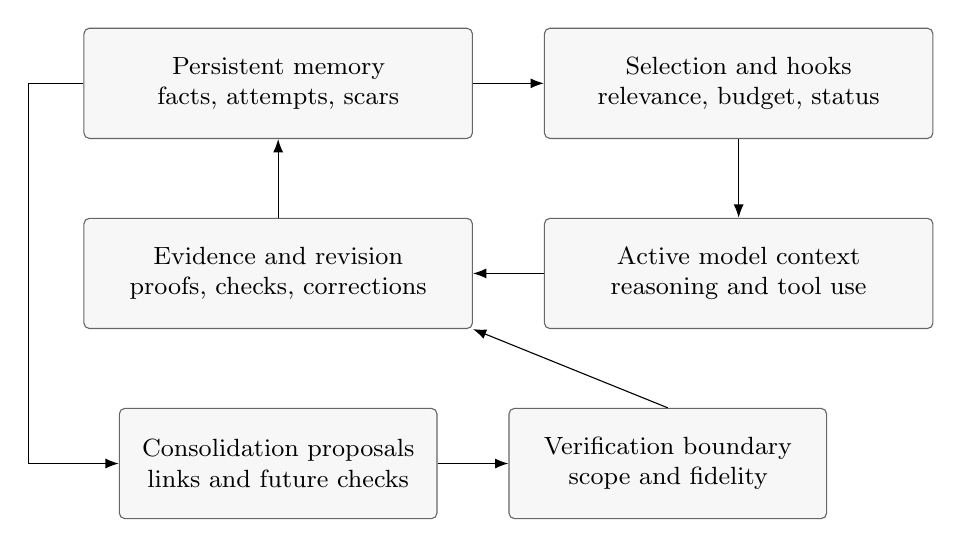
\begin{tikzpicture}[node distance=10mm and 9mm,>=Latex,
 box/.style={draw=black!60,rounded corners=2pt,fill=black!3,align=center,text width=38mm,minimum height=14mm,font=\small},
 wide/.style={box,text width=47mm}]
\node[wide] (memory) {Persistent memory\\facts, attempts, scars};
\node[wide,right=of memory] (retrieve) {Selection and hooks\\relevance, budget, status};
\node[wide,below=of retrieve] (context) {Active model context\\reasoning and tool use};
\node[wide,left=of context] (evidence) {Evidence and revision\\proofs, checks, corrections};
\node[box,below=of evidence] (replay) {Consolidation proposals\\links and future checks};
\node[box,right=of replay] (verify) {Verification boundary\\scope and fidelity};
\draw[->] (memory)--(retrieve);
\draw[->] (retrieve)--(context);
\draw[->] (context)--(evidence);
\draw[->] (evidence)--(memory);
\draw[->] (memory.west) -- ++(-7mm,0) |- (replay.west);
\draw[->] (replay)--(verify);
\draw[->] (verify.north)--(evidence.south east);
\end{tikzpicture}
\caption{Operational conscious--subconscious cycle. Consolidation proposes work; verification controls the evidentiary status of what returns to memory. Arrows describe the architecture, not proof that every deployment completes every stage.}
\label{fig:cycle}
\end{figure}

The surrounding system and the specialized Math Brain should be distinguished. The former includes broad memory, user context, operational reminders, and coordination. The latter isolates mathematical objects and verification rules. A comparison of the entire surrounding system against a minimal context measures a bundled intervention. It does not isolate the contribution of mathematical memory or any particular hook.

\Needspace{6\baselineskip}
\subsection{Memory layers}

\begin{longtable}{p{0.20\linewidth}p{0.33\linewidth}p{0.39\linewidth}}
\caption{Memory layers and their computational purpose. Sources: \citep{broadarchitecture,matharchitecture,consciousness,canonical}.}\\
\toprule
Layer & Representation & Function and evidentiary boundary\\
\midrule
\endfirsthead
\toprule Layer & Representation & Function and evidentiary boundary\\ \midrule
\endhead
Episodes and history & Session records, prompts, prior revisions & Recover what happened. An utterance is evidence that it was made, not that it was correct.\\
Reusable memory & Dated topic records with descriptions and metadata & Preserve methods, decisions, rationale, and corrections across contexts.\\
Navigation & Indexes, topic maps, links, backlinks & Find the relevant record without loading the whole archive.\\
Salience & Recency, curation, type, graph centrality, consequence scores & Allocate attention. High importance does not raise truth status.\\
Mistakes and scars & Failure mechanism, minimal failing step, repair, counterexample & Preserve negative knowledge and prevent a refuted route from being rediscovered as new.\\
Instincts and reflexes & Cue, ordered checks, required evidence, stop condition & Turn a lesson into a targeted action at the time it matters.\\
Mathematical objects & Definitions, claims, examples, lemmas, conjectures, proof attempts & Preserve quantifiers, hypotheses, constants, regimes, and exact dependencies.\\
Evidence & Calculations, proof artifacts, citation locators, formal receipts & Support a particular claim revision at a stated scope.\\
Consolidation & Review agenda, gists, link proposals, counterexample tasks & Compress and connect records; proposed content remains subject to verification.\\
Coordination & Leases, identities, handoffs, current work & Identify present ownership and progress. This state is distinct from durable mathematical knowledge.\\
\bottomrule
\end{longtable}

This layering addresses different failure modes. Episodic history prevents a summary from erasing the reason for a correction. Typed mathematics prevents a theorem from losing an essential hypothesis. Scar memory prevents a counterexample from becoming an inaccessible footnote. Navigation and salience keep useful material accessible under a finite context. Coordination reduces duplicated effort but cannot certify the mathematics produced by the workers.

\subsection{Hooks and delivery}

A hook is a program invoked at a lifecycle event. The inspected settings route session start, prompt submission, pre-tool activity, post-tool activity, and session termination to appropriate handlers. A wake routine supplies continuity at session start. Prompt hooks can surface a relevant memory or mathematical card. Pre-tool hooks can warn before an action with a known failure mode. Post-tool hooks observe errors or co-read memories. Stop hooks retain unresolved obligations and continuation information \citep{dispatcher,wake,instincts,mathsense,proofhooks}.

These event boundaries are useful because the same information has different value at different times. A warning about a denominator is useful immediately before division; a warning about an unproved exchange of limits belongs near the limiting argument; a reminder to bind a proof to its source revision belongs near verification and publication. Repeating every warning in every prompt wastes context and can reduce attention to the relevant one.

The source records a concrete delivery limit: 646 of 1,009 prompt merges in one historical interval exceeded an inline bound, with a median payload near 53 KB. The revised dispatcher uses a 9,800-character inline allocation and retains overflow separately. Its water-filling policy preserves short messages and shortens large ones to available shares. Wake output is divided into two bounded parts \citep{dispatcher,wake}. These are character budgets, which must not be reported as model-token counts without a specified tokenizer.

The pipeline must be evaluated at successive boundaries: stored, indexed, retrieved, emitted, delivered, acted on, and outcome verified. Passing an early boundary does not establish the later ones. The mathematical-card hook illustrates the importance of this distinction. Its September 22 source diagnosis records 710 silent real-session invocations between September 15 and 22 because NumPy was unavailable under the dispatcher's invocation mode, while ordinary-Python harness tests served cards. A source repair was added. This supports a documented deployment-path failure and repair; current end-to-end recovery still requires an observed delivery record \citep{mathsense}.

\subsection{Policy routes, pinned memories, and bounded delivery}
\label{sec:policy_delivery_update}

The September 23 source update makes explicit routing part of candidate generation. A recall-policy entry has one of three modes: \texttt{normal}, \texttt{parent\_only}, or \texttt{disabled}. Parent-only routes require their approved direct lexical or intent condition, while disabled entries are removed from ordinary deliberate retrieval. The new behavior lets a normal entry carry multi-term trigger groups and explicit token aliases. When every term of any group occurs in the alias-enriched query and no configured blocking phrase matches, the entry receives a policy seed of strength $3$ and a lexical seed of at least $3$. Without a trigger, it retains ordinary retrieval eligibility. This mechanism is a hand-authored routing rule; matching a reviewed spelling or token group does not establish semantic generalization \citep{brainrecall20260923,recallpolicy20260923}.

Policy precedence also required a repair. The original promotion placed a policy seed above the initial BM25 peak by an additive margin. Later multiplicative name-coverage and question-coverage boosts could move an ordinary result above it. The revised default BM25-first path lifts policy candidates again after those boosts. Writing $b_j$ for the adjusted non-policy scores and $s_i$ for a policy strength, the implemented lift is
\[
 b_i^{\mathrm{policy}}
 = \max_{j\notin P} b_j + 2 + \frac{s_i}{s_{\max}},
\]
with a fallback to the initial BM25 peak when there is no non-policy score. This restores precedence at that stage while retaining policy-strength order. It is a scoped implementation property: \texttt{BRAIN\_RECALL\_BLEND=1} selects the legacy blend, and the later optional status-order pass can rerank candidates; that pass defaults to off. A change to a subsequent ranking stage therefore requires another precedence check \citep{brainrecall20260923}.

Pins have an opportunity cost. Deliberate recall defaults to eight displayed rows, and a pinned entry occupies an ordinary row in that allowance. Moreover, the seed is inserted before graph propagation and seed-based semantic expansion. The implementation consequently does not guarantee that removing the pinned row would recover an otherwise identical result list. Such preservation must be measured on a stated query set. The pin switch, \texttt{BRAIN\_RECALL\_PINS=0}, disables the new normal-entry promotions. Independently, displayed descriptions now prefer the memory's own frontmatter, read from a bounded prefix, and default to a 320-character excerpt with an ellipsis when shortened \citep{brainrecall20260923}.

Delivery imposes further limits beyond retrieval rank. The dispatcher retains its 9,800-character allocation, whereas owner-history delivery defaults to a 9,000-UTF-8-byte budget after accounting for existing context and its history notice. These quantities are not model-token counts. The new dispatcher can skip ten designated operational hooks for recognized headless workers when its marker is present, and avoids launching a hook whose explicit enabling file is absent. These controls specify conditional source behavior; source presence does not establish which marker or settings a deployed session used \citep{dispatcher20260923,ownerdelivery20260923}.

The evidence boundary remains explicit. Owner-history state records a context hash and byte length only after successful stdout writing and flushing, labeling the receipt \texttt{emitted\_stdout\_not\_receiver\_verified}. Retrieval and emission therefore require separate evidence from receipt, action, and outcome. Similarly, the revised regression gate accepts selected growing-input receipt differences within a default three-hour window, while still rejecting other source-field drift. A passing freshness check under that rule is compatible with limited input growth; it is not an assertion that every source field is identical to the build snapshot \citep{ownerdelivery20260923,braingate20260923}.


\subsection{Salience and memory precedence}

The implemented salience rule combines recency and persistence using a noisy-OR form:
\begin{align}
R_i &= \exp(-a_i/\tau),&
P_i &= 1-\prod_j(1-c_{ij}),&
S_i &= 100\bigl[1-(1-R_i)(1-P_i)\bigr].
\label{eq:salience}
\end{align}
Here $a_i$ is age in days, and the components $c_{ij}\in[0,1]$ encode such signals as curation, backlinks, record type, and lexical consequence. The default recency parameter in the inspected code is $\tau=1.3$ days, with a rollback option to an earlier 45-day parameter. Example component values include 0.80 for curation and type priors of 0.90 for feedback/user records, 0.16 for reference records, and 0.07 for project records. Supersession reduces priority while preserving history \citep{salience}.

The shape gives an enduring record a persistence floor even when its recency fades. These bounded scores are ranking heuristics, not calibrated probabilities of truth. Their historical calibration used 1,391 deliberate recall reads over 26 days, joined to 2,523 creation dates. Reported rates decrease sharply for new memories and then flatten, with a nominal short timescale of 1.3 days and a much slower tail. The study itself notes that observed reads depend on the existing retrieval policy \citep{recency}. Thus the fitted curve estimates use under that policy; it is not an intrinsic forgetting law.

An audit also found a mismatch between the salience parameter and the legacy precedence classifier. A fixed recency threshold of 0.72, documented under $\tau=45$ days, corresponds under $\tau=1.3$ to an age of $-1.3\log(0.72)\approx0.427$ days. A threshold of 0.40 corresponds to about 1.191 days. Eligible short, uncurated project memories could therefore be demoted much sooner than the older comments imply. Curation and other exception paths limit the affected set \citep{consciousnesscode,salience}. This is an example of parameter coupling that a formal dynamics model can make explicit.

\subsection{Associations and pattern recognition}

Co-reading provides one association signal. The inspected fold procedure keeps at most 40 distinct memories per session. A fold decays existing weights by 0.98 and adds $\min(1,6/n_s)$ to a co-read pair from a session containing $n_s$ memories, followed by a pruning floor. It uses stable identities and receipts to avoid replaying the same fold as fresh evidence \citep{coactivation}. The decay is event-based. A busier fleet can therefore change the wall-clock retention rate even if the same decay parameter remains in the code.

The live general association hook performs two hops of degree-normalized propagation. In a source-faithful abstraction, an edge contribution is
\[
f_{i\to j}^{(h+1)}
=0.5\,a_i^{(h)}
\frac{w_{ij}}{\sum_k w_{ik}}
(1+0.4s_j)\gamma_j,
\]
where $s_j$ is a severity signal and $\gamma_j$ is a possible topic gain. Repetition controls, salience thresholds, winner margins, supersession routing, and near-duplicate suppression determine whether a candidate is shown. Its trace retains the contributing bridge \citep{spread}. Multiplying every outgoing weight at a node by the same positive constant leaves its normalized transition probabilities unchanged. More stored edge weight is consequently not, by itself, more effective retrieval.

Mathematical retrieval adds notation-normalized tokens, alpha-renamed formula fingerprints, and typed graph edges. Normalization helps match different variable names; it is not a theorem that two expressions are mathematically equivalent. An optional semantic channel uses normalized embedding vectors and positive standardized cosine scores. The live mathematical-card hook also uses lexical prefiltering and compact rendering, and labels population-store cards with their secondary or unverified provenance \citep{mathretrieval,semantic,mathsense}.

The system makes a valuable distinction between \emph{discovery} and \emph{proof dependency}. Discovery may traverse analogy and semantic similarity. A proof must identify exact assumptions and directed premises. The exact dependency-closure routine follows only the designated dependency edges and rejects missing nodes or cycles. Negative edges such as refutations receive positive visibility but retain a negative evidentiary meaning. A nearby counterexample should be easy to find without being mistaken for support \citep{matharchitecture}.

\subsection{Scars, instincts, and calibrated warnings}

A scar is a persistent record of a failure and its generating condition. An instinct is a compiled cue-to-check policy. The mathematical mistake schema includes the claim, failure class, minimal bad step, cause, repair, affected assumptions, and optional counterexample. Its reflex schema adds activation cues, ordered checks, required evidence, and an explicit stopping condition \citep{mistakes,triggers}.

Examples include requiring a nonzero denominator, checking a sign after squaring, naming the convergence theorem before exchanging limits, writing quantifiers and their negations, and distinguishing a finite computation from a universal argument. A useful scar says why a step fails and when that reason applies. A vague instruction to be careful has little diagnostic value.

Warnings can also be harmful. They can interrupt a sound proof, retrieve an analogy whose hypotheses differ, or cause an agent to reject a valid argument because it resembles an old failure. The broad instinct layer ranks and limits warnings, records the triggering channel, and suppresses repeated delivery \citep{instincts}. In an internal study of 91 corrections, graph clustering produced groups whose modularity was not unusual under a degree-preserving null (reported $z\approx-0.9$). Those groups can organize records without constituting established natural classes of mistakes \citep{mistakegraph}.

\subsection{Familiarity, forecasts, and self-monitoring}

The feeling-of-knowing probe searches descriptions and filenames before reading complete memory bodies. It uses distinctive terms, bounded typo correction, and a cluster threshold, with salience as a secondary ranking signal. Its appropriate interpretation is that the corpus appears to contain relevant material. It is not evidence that the model knows a theorem or can prove it. The inspected probe is expressly silent on mathematical arguments, leaving that task to specialized proof routing \citep{fok}.

The forecasting component stores dated probabilities and resolves them against observed outcomes. It uses Brier loss $(p-o)^2$ and realized self-information $-\log_2 p_o$. A per-scope hit rate is shrunk toward a global base rate $g$ as $(h+4g)/(n+4)$, with small samples marked provisional \citep{prediction}. These scores can evaluate forecasts about runtime reliability or a task outcome. They are not proof probabilities for mathematical theorems.

The architecture also uses signals described as affect, charge, surprise, danger, or conscience. Their operational roles are attention, routing, rechecking, persistence, and stopping. This separation matters: a high-consequence failure may warrant stronger review without making the remembered factual claim more probable. Repeated surprise can justify examining an alternative model; it cannot determine a theorem's truth by itself \citep{broadarchitecture,canonical,reconsolidation}.

\subsection{Consolidation and coordination}

The general system uses background agendas and model-assisted synthesis to produce gists, links, and review tasks. The mathematical package imposes a stricter boundary: its deterministic consolidation function returns quarantined proposals. Contradictions, missing evidence, reflex rehearsal, isolated nodes, and hub review receive explicit priorities. Analogy proposals use abstract mathematical structure, but cannot promote themselves to verification evidence \citep{consolidation}.

The agent mesh separately tracks identities, leases, current tasks, messages, and acceptance of handoffs. Durable lessons pass through a memory-writing interface; routine activity remains transient coordination. A separate global-workspace component has source and design documentation, but its wiring record still reports an uncompleted integration gate. Current broadcast deployment is therefore not established by those files \citep{mesh,globalworkspace}.

The current mathematical repository describes itself as a coordination archive and explicitly does not claim native ingestion of newly produced research across all scheduled runtimes. This is compatible with historical experiments using a local populated store. Version, corpus, runtime, and delivery evidence must therefore accompany any assertion that an agent was connected to Math Brain \citep{mathreadme}.

\section{A mathematical framework for pseudo-cognitive dynamics}
\label{sec:dynamics}

This section formalizes the architecture and derives consequences under stated assumptions. Some equations describe implemented rules; other operators are proposed abstractions. None of the propositions establishes an empirical improvement in mathematical ability. Their purpose is to make budgets, stability, evidence flow, and possible failure modes explicit.

\subsection{State, retrieval, and external learning}

\begin{definition}[Pseudo-cognitive state]
At event time $t$, let
\[
Z_t=(C_t,M_t,W_t,G_t,L_t).
\]
Here $C_t$ is the active context, $M_t$ the persistent memory records, $W_t$ an association graph, $G_t$ the mathematical claim and evidence graph, and $L_t$ an append-only event and resource ledger. The context has serialized token length $\ell(C_t)\leq B$. A memory record contains content, applicability conditions, provenance, a revision identifier, and an evidence state.
\end{definition}

An event $e_t$ may be a question, tool result, error, checkpoint, or scheduled review. A hook generates a query and available memory budget. Retrieval and packing give
\[
q_t=H(e_t,C_t),\qquad
R_t=\mathcal{R}(q_t,M_t,W_t,G_t;b_t),\qquad
\widetilde C_t=\operatorname{Pack}_{B}(C_t,R_t).
\]
The model generates an action $a_t\sim\pi_\theta(\,\cdot\mid\widetilde C_t)$; observations and checks then update external state:
\[
(M_{t+1},W_{t+1},G_{t+1},L_{t+1})
=U(Z_t,e_t,R_t,a_t,y_t,V(y_t)).
\]
In this model $\theta$ is fixed. Learning occurs through external records, associations, retrieval policies, and procedures. External learning and model-weight training are different resource and attribution categories.

A retrieval budget should include the serialized wrapper and metadata, not only the body of a memory. If mandatory context has length $m_t$ and response reserve $o_t$, the available budget is $b_t=B-m_t-o_t$. It exists only when this quantity is nonnegative. A packing operator that accepts a block only after checking the length of the full resulting serialization preserves $\ell(\widetilde C_t)+o_t\leq B$ by induction over accepted blocks. This simple invariant prevents silent budget overflow; it says nothing about the quality of what was retained.

\subsection{Salience is bounded and saturating}

\begin{proposition}[Noisy-OR salience]
For $c_1,\ldots,c_m\in[0,1]$, let
$F(c)=1-\prod_{j=1}^m(1-c_j)$. Then $F\in[0,1]$, is coordinatewise nondecreasing, and the increment from adding a further component $d\in[0,1]$ is
\[
F(c_1,\ldots,c_m,d)-F(c_1,\ldots,c_m)
=d\prod_{j=1}^m(1-c_j).
\]
This increment decreases when any existing component increases.
\end{proposition}
\begin{proof}
Every factor $1-c_j$ lies in $[0,1]$, proving the bounds. Increasing a component decreases the residual product. The displayed identity follows by factoring that product, and proves the final assertion.
\end{proof}

Equation~\eqref{eq:salience} is of this form, with recency as an additional component and a scale factor of 100. A union-probability interpretation would require suitable independence assumptions; the ranking rule does not supply them. In particular, backlinks, repeated reading, and curation can be correlated consequences of the same original attention. Treating their combined salience as independent verification would count the same evidence repeatedly.

\subsection{Association growth and time}

\begin{proposition}[Forgetting with bounded reinforcement]
Let $w_{t+1}=\rho w_t+\eta_t$, where $0\leq\rho<1$, $w_0\geq0$, and $0\leq\eta_t\leq K$. Then
\[
w_t=\rho^tw_0+\sum_{j=0}^{t-1}\rho^{t-1-j}\eta_j
\leq \rho^tw_0+K\frac{1-\rho^t}{1-\rho}.
\]
\end{proposition}
\begin{proof}
Repeated substitution gives the equality. Bounding each reinforcement by $K$ and summing the geometric series gives the inequality.
\end{proof}

For a single-session reinforcement bounded by one and decay $\rho=0.98$, the limiting bound is 50. If a fold processes several sessions, $K$ must bound their total contribution; one must not apply the single-session numerical bound to an arbitrarily large batch. Pruning can reduce the bound but does not establish a fixed wall-clock forgetting rate.

Suppose an unreinforced weight undergoes $N(T)$ folds during a physical interval of length $T$. Its value becomes $\rho^{N(T)}w_0$. Thus two fleets with different fold counts forget at different rates even under identical parameters. A proposed time-normalized alternative is
$w(t+\Delta)=e^{-\lambda\Delta}w(t)+\eta(t,\Delta)$.
This keeps the passive decay independent of event frequency, but the usefulness of either rule requires a matched comparison.

\subsection{Stable activation under a sufficient condition}

\begin{proposition}[Contractive activation]
Let $P$ be a nonnegative matrix with every row sum at most one. Let $\sigma:\mathbb{R}^d\to\mathbb{R}^d$ be coordinatewise clipping to $[0,1]$. For fixed $b$ and $0\leq\alpha<1$, define
\[
T_b(a)=\sigma(\alpha Pa+b).
\]
Then $T_b$ has a unique fixed point $a^\ast(b)$, iterations converge to it, and
\[
\norm{a^\ast(b)-a^\ast(b')}_\infty
\leq \frac{\norm{b-b'}_\infty}{1-\alpha}.
\]
\end{proposition}
\begin{proof}
Clipping is nonexpansive and $\norm{P}_\infty\leq1$. Therefore
$\norm{T_b(a)-T_b(a')}_\infty\leq\alpha\norm{a-a'}_\infty$.
The cube $[0,1]^d$ is complete, so the contraction theorem gives a unique fixed point and convergence. For two fixed points, the triangle inequality gives
$\norm{a^\ast(b)-a^\ast(b')}_\infty
\leq\alpha\norm{a^\ast(b)-a^\ast(b')}_\infty+\norm{b-b'}_\infty$.
Rearranging proves the sensitivity bound.
\end{proof}

This is a sufficient-condition model, not a convergence theorem for every inspected hook. The actual two-hop rule contains severity and topic gains, which can destroy the stated row-sum bound; it also stops after a finite number of hops. The distinction is useful: a proposed indefinitely iterated activation process must control total gain, while a finite-depth search must control depth, candidate count, and score sensitivity.

If all final candidate scores change by at most $\varepsilon$, a unique winner whose original margin exceeds $2\varepsilon$ remains the winner. Indeed, its decrease is at most $\varepsilon$ and a competitor's increase is at most $\varepsilon$. This elementary fact explains why explicit winner margins can stabilize retrieval, although it does not establish that the chosen memory is correct.

\subsection{Selecting useful context under a budget}

Consider a finite set of candidate cards and a task with a finite set of nonnegative-weight obligations $u\in\mathcal U$. A memory card $i$ is assigned coverage $a_{ui}\in[0,1]$. As a proposed approximation to useful coverage, define
\[
F(S)=\sum_{u\in\mathcal U}v_u\max_{i\in S}a_{ui},
\qquad F(\varnothing)=0,\quad v_u\geq0.
\]
Repeated cards about the same obligation produce diminishing gains. This model does not include misleading cards or synergistic proofs requiring several premises simultaneously; those effects require a richer objective.

\begin{proposition}[A standard greedy guarantee for the coverage model]
For an integer $k\geq1$, repeatedly add a card of largest marginal increase in $F$, until $k$ cards have been selected or no candidate remains. Early stopping is also allowed when every remaining marginal gain is zero. If $S_g$ is the resulting set and $S^\ast$ maximizes $F$ among sets of size at most $k$, then
\[
F(S_g)\geq\bigl[1-(1-1/k)^k\bigr]F(S^\ast)
\geq(1-e^{-1})F(S^\ast).
\]
\end{proposition}
\begin{proof}
The maximum for each obligation is nondecreasing as cards are added. Its marginal gain from adding a fixed card decreases as the selected set grows. Hence $F$ is monotone and submodular. At any step with selected set $S_j$, submodularity and monotonicity give
$F(S^\ast)-F(S_j)\leq\sum_{i\in S^\ast\setminus S_j}
[F(S_j\cup\{i\})-F(S_j)]$.
There are at most $k$ terms. Greedy therefore gains at least
$(F(S^\ast)-F(S_j))/k$. Iterating the resulting deficit inequality from $F(S_0)=0$ proves the first bound. The inequality $(1-1/k)^k\leq e^{-1}$ proves the second.
\end{proof}

This is the classical cardinality-constrained submodular argument \citep{nemhauser1978}, applied to a proposed context-selection model. It is not a new optimization theorem and not an established model of this system's real utility. It applies directly to equal-cost slots. Arbitrary token lengths create a knapsack constraint, for which the same simple cardinality proof does not apply. Harmful or complementary information can also violate monotonicity or submodularity. These limitations matter more than the attractive approximation constant.

\subsection{Proof dependencies and correction propagation}

\begin{proposition}[Compositional assumption tracking]
Let a finite acyclic graph represent exact formal propositions. Suppose each node $v$ has a checked derivation of $P_v$ from its immediate premises and a recorded assumption set $A_v$. Then $P_v$ follows from the union of $A_u$ over the premise ancestors of $v$, including $v$.
\end{proposition}
\begin{proof}
Order the graph topologically. At a node without premises, the conclusion follows from its own assumptions by hypothesis. At a later node, substitute the already established premise derivations into its checked derivation. The required assumptions are contained in its own set and the ancestor sets of its premises. Induction proves the claim.
\end{proof}

This standard composition principle clarifies why the memory representation must preserve hypothesis direction and statement identity. A formally checked implication containing the desired theorem as a hypothesis is still conditional.

When a premise revision is refuted or withdrawn, the appropriate response is to flag the derivations that depend on that revision for revalidation. The smallest such set closed under downstream dependency is its reachable dependent set: reachability is closed, and any closed set containing the changed node must contain every node along each path. Marking that set does not prove all those conclusions false. Another proof may survive, a stronger premise may be unnecessary, or a replacement revision may repair the derivation. Revision-specific dependency tracking preserves those distinctions.

\subsection{When a scar can help}

Suppose a narrowly defined warning is relevant with probability $p$ on a specified task distribution. Conditional on relevance, it prevents a failure with probability $r$ and avoided loss $L$. On irrelevant cases it causes a harmful intervention with probability $f$ and loss $H$. If delivery has cost $c$ in the same utility units, its expected net value in this simplified model is
\[
V=prL-(1-p)fH-c.
\]
The warning is beneficial exactly when this expression is positive. This identity makes specificity, uptake, false alarms, and overhead separate measurable quantities. A count of delivered warnings does not estimate any one of them.

\subsection{Selective warnings under a context budget}
\label{sec:warningbudget}

The single-warning value identity does not account for warnings that detect the same failures. A small decision model makes that interaction explicit. It concerns proof-audit verdicts, not theorem discovery, and its parameters are illustrative rather than fitted to the experiments.

Let $V$ be the event that an audited proof is valid, with $\Pr(V)=\pi\in(0,1)$. Each candidate warning has an alert event $F_i$ on a common probability space. Assume that these events do not change when other cards are selected. For a selected set $S$, the auditor rejects the proof if any selected warning alerts, and otherwise accepts it. Thus a false alert can reflect an applicability mistake even when the stored warning is mathematically sound. Write $E_S=\bigcap_{j\in S}F_j^c$, with $E_\varnothing$ the entire sample space. The probability of a correct verdict is
\[
 A(S)=\pi\Pr(E_S\mid V)
 +(1-\pi)\bigl[1-\Pr(E_S\mid V^c)\bigr].
\]
A correct audit verdict can be either acceptance of a valid proof or rejection of an invalid one.

\begin{proposition}[Marginal value of an additional warning]
For $i\notin S$, without any independence assumption,
\begin{align*}
 A(S\cup\{i\})-A(S)
 ={}&(1-\pi)\Pr(E_S\cap F_i\mid V^c)\\
 &-\pi\Pr(E_S\cap F_i\mid V).
\end{align*}
\end{proposition}
\begin{proof}
Since $E_{S\cup\{i\}}=E_S\setminus F_i$, subtracting the two expressions for $A$ gives the identity. The only verdicts that change are those on which all previous warnings remain silent and the additional warning alerts. On invalid proofs this change is a correction; on valid proofs it is an error.
\end{proof}

Consequently, a warning's detection rate on all invalid proofs is insufficient to determine its incremental value. It must detect failures missed by the selected warnings. A perfect duplicate of an existing alert has zero marginal accuracy. More strongly, if it detects no previously missed invalid proofs but creates a new false alert with positive conditional probability, its marginal accuracy is strictly negative. These statements allow arbitrary dependence among alerts under the stated common-response assumption.

\begin{proposition}[Optimal count of interchangeable warnings]
Suppose there are $N$ warning cards whose alerts are mutually independent conditional on $V$ and also conditional on $V^c$. Each has false-positive probability $f=\Pr(F_i\mid V)$ and detection probability $d=\Pr(F_i\mid V^c)$, where $0<f<d<1$. If every card has the same fully serialized token length $\tau>0$ and available memory budget is $b\geq0$, let $k=\min\{N,\lfloor b/\tau\rfloor\}$. Then selecting $n\leq k$ cards gives
\[
 A_n=\pi(1-f)^n+(1-\pi)\bigl[1-(1-d)^n\bigr].
\]
Define
\[
 t=\frac{\log\!\bigl((1-\pi)d/(\pi f)\bigr)}
 {\log\!\bigl((1-f)/(1-d)\bigr)}.
\]
The smallest accuracy-maximizing feasible count is
\[
 n^\ast=\min\{k,\max\{0,\lceil t\rceil\}\}.
\]
If $t$ is a nonnegative integer and $t+1\leq k$, the adjacent count $t+1$ is also a maximizer.
\end{proposition}
\begin{proof}
Conditional independence gives the two probabilities of silence as products, proving the formula for $A_n$. Subtraction gives
\[
 A_{n+1}-A_n
 =(1-\pi)d(1-d)^n-\pi f(1-f)^n.
\]
Both terms on the right are positive before subtraction. Their ratio is
\[
 \frac{(1-\pi)d}{\pi f}
 \left(\frac{1-d}{1-f}\right)^n.
\]
It strictly decreases with $n$, and equals one precisely when $n=t$. Thus the increments are positive for $n<t$, zero for $n=t$, and negative for $n>t$. Truncating the resulting maximizing count to the feasible interval $\{0,\ldots,k\}$ proves the claim, including its tie case.
\end{proof}

For example, take $\pi=4/5$, $d=4/5$, and $f=1/20$, with room for at least three cards. The correct-verdict probabilities for zero, one, two, and three warnings are respectively
\[
 0.8000,\qquad 0.9200,\qquad 0.9140,\qquad 0.8843.
\]
Every warning improves accuracy when supplied alone, yet adding the second warning lowers accuracy. The earlier warnings have already detected most invalid proofs, while further warnings still create false rejections. In this example one card is optimal despite the larger available budget. The monotone coverage guarantee above therefore does not transfer to this audit objective. If the larger packet also has higher positive mean operating cost, the smaller packet has lower cost per correct verdict, using the common-population criterion in Section~\ref{sec:costs}.

These are elementary probability calculations, not a new theorem about optimal inference. An evaluator allowed to ignore additional information can retain its former decision policy; the example instead concerns a specified response rule. Conditional independence, equal diagnostic quality, and fixed alert behavior are strong assumptions. Actual memory can alter interpretation, repair an argument, expose a new proof, or displace other context. A full-versus-diet comparison cannot identify the mechanism from packet size and final score alone. It should record which additional cards detect previously missed errors, which cause false rejections, and their delivery and verification costs. The model demonstrates one possible reason for selective delivery, without asserting that it explains an observed treatment contrast.


\section{Lean, algorithms, and mathematical audits}
\label{sec:verification}

\subsection{The division of responsibility}

Memory helps a mathematical audit by recovering relevant definitions, theorem hypotheses, earlier failures, and precise source locations. The model still has to decide whether they apply. Numerical tools test examples and find counterexamples; symbolic tools establish identities within their domains; Lean checks an encoded statement against its formal dependencies; a fidelity review compares that statement with the intended mathematics. These activities support different conclusions \citep{leanref,leanarchitecture}.

For example, a finite search can refute a universal statement by finding one valid counterexample. A finite search with no counterexample proves a universal claim only if it exhausts the admissible domain or a complete reduction to that search is established. A failed Lean tactic can reflect an unavailable lemma, syntax error, timeout, or poor proof search; it does not refute the target theorem. A successful Lean proof can establish a weaker or different theorem than the prose if the translation is wrong.

The archive's specialized proof hook converts recurring failure types into a small audit packet. It selects cues involving named-theorem applicability, inequality direction, quantifiers, constants, load-bearing assumptions, and limiting targets, and produces a step inventory. It limits repeated delivery and explicitly warns that retrieved notes themselves require applicability checks \citep{proofhooks}. This is a direct operational example of subconscious-to-conscious transfer: previous errors determine what the next audit is prompted to inspect.

\subsection{The isolated mathematical authority}

The isolated package has an unusually strict formal-verification path. Its inspected project pins Lean 4.30.0 and accepts a narrowly defined local source graph. It stable-reads and snapshots source bytes, uses a direct pinned executable, compiles in dependency order, records exact declaration names, and binds source, toolchain, execution, and output identities. The authority route requires canonical axiom reports for the named declarations and an empty reported axiom set \citep{leanarchitecture,leanimplementation}.

This policy is stricter than common Mathlib use. It is therefore misleading to merge the package's rule with every research companion and call the whole project an axiom-free Lean system. The package's own small formal library contains three elementary natural-number controls. Those controls exercise the verification mechanism; they are not a formalization of the research programme \citep{leannatural,leancontrols}.

The package separates automated kernel evidence from formalization-fidelity evidence. The latter records review of quantifiers, domains, definitions, assumptions, conclusions, boundary cases, and extra assumptions. The records are bound to exact claim and source revisions. Cryptographic receipts can bind those fields to an issuance path, but do not make an inaccurate human translation correct. Imported peer reports remain discovery material until the appropriate local verification path supplies evidence \citep{leanimplementation,matharchitecture}.

\subsection{The broader Mathlib checker}

The surrounding brain has a different checker using a local Mathlib project. Its parser permits the conventional Lean axioms \code{propext}, \code{Classical.choice}, and \code{Quot.sound}, while rejecting placeholders such as \code{sorryAx} and custom axioms. Its receipt retains an unverified translation-fidelity field. This path supplies valuable formal evidence, but its assurance conditions differ from those of the isolated package \citep{leanbroad,leanparser}.

The distinction can be expressed as three questions. Did the intended executable check the exact source? What proposition and assumptions did it check? Does that proposition faithfully express the research claim? The first is execution provenance, the second formal correctness, and the third semantic fidelity. A rigorous audit records all three.

\begin{table}[htbp]
\centering\small
\begin{tabularx}{\linewidth}{p{0.25\linewidth}rYY}
\toprule
Inspected companion & Named reports & Checked content & Remaining scope\\
\midrule
Free unimodality & 13 & Polynomial/rational identities, profile bounds, equality cases & Probability measures, free convolution, parametrization, full theorem\\
Arc-transitive graphs & 17 & Blow-up arithmetic, cycle sums, hitting-mass formulas & Identification with stochastic quantities and graph hypotheses\\
Degree counts & 17 & Stage arithmetic, mass and centering bounds, exponent identities & Full conditional probability argument and limiting statement\\
Bernoulli convolution & 25 & Separate seven-file summary of conditional algebra/analysis & One-copy absolute continuity and the unresolved contraction step\\
\bottomrule
\end{tabularx}
\caption{Representative formal evidence. Counts are distinct named declarations in inspected axiom-report records, not counts of solved problems or necessarily every declaration in the files. The first three total 47. Sources: \citep{freelean,arclean,degreelean,bc23lean}.}
\label{tab:lean}
\end{table}

These companions show a practical use of formalization even when an entire research proof is not encoded. A delicate coefficient identity or polynomial inequality can be isolated and checked. That removes one class of algebraic uncertainty and allows the informal review to focus on measure-theoretic hypotheses, conditioning, limiting arguments, and interpretation. The value comes from knowing which part was checked.

\subsection{Environment-specific integration}

Inspected scheduled records from September 21 report missing Lean and mathematical-package dependencies in several Linux accounts. Some records show zero of three genuine formal controls completed while a synthetic containment or executable-transport test passed. The production POSIX lease in the inspected isolated implementation also marks executable locking as unenforced, which prevents authority eligibility under its own rules \citep{leanblocked,leanimplementation}.

These are dated, environment-specific observations. They coexist with successful research-companion build logs elsewhere. They justify neither a claim that Lean never worked nor a claim that all workers were fully connected. A formal-system audit must identify the machine or runtime, exact toolchain, source revision, named declarations, dependency assumptions, and receipt.

For this paper, 11 local receipt-parser controls and a proof-hook routing check with one positive and two negative inputs were run successfully. These checks test parsing and routing. A Lean executable was unavailable in the review environment, so the historical kernel checks were inspected rather than rerun. The reproduction supplement records that boundary.

\subsection{A complete audit workflow}

A useful workflow begins with an exact mathematical statement and an obligation inventory. Each obligation receives an appropriate check, and each check records its scope. A proof that depends on an external theorem retains that theorem's source, statement, and hypotheses. A counterexample is stored with admissibility conditions. A formalization retains its informal counterpart and any extra assumptions. A correction creates a new revision and triggers review of dependent derivations.

Independent review is strongest when the reviewer reconstructs a load-bearing step from the original assumptions or uses a different method. Several agents repeating the same derivation can detect typographical errors, but agreement does not eliminate a shared conceptual mistake. Likewise, a majority vote is a record of opinions, not a proof. The architecture's evidence graph is useful precisely because it can preserve the source of each review instead of reducing all agreement to one confidence score \citep{canonical,matharchitecture}.

Memory supports this workflow through continuity and targeting. It can warn that a previous argument reversed an inequality, that a formal lemma assumed the desired conclusion, or that a conditioning step destroyed independence. The audit must then test the warning against the current argument. A sound use of scars is to focus attention on a possible failure, followed by a mathematical decision.

\section{Evaluation methods and observed performance}
\label{sec:eval}

\subsection{What each kind of test measures}

The archive contains several different evaluation families. Retrieval tests ask whether a target record appears in the returned set. Private-knowledge tests ask for facts or source locations available in the project's memory. Proof-audit tests ask whether a mathematical argument is valid and, if not, where it first fails. Scar tests ask whether an agent avoids a known practical trap. Infrastructure tests exercise schemas, isolation, parsers, provenance, or runtime delivery.

These endpoints should not be merged into one accuracy number. A system can retrieve a remembered answer perfectly without improving deduction on an unseen theorem. It can pass a parser test while a production hook fails to import a dependency. It can improve recall while increasing total cost. The methodology must preserve the question each test was designed to answer.

A planted-error bank typically begins with a correct proof, changes a line or assumption, and asks the solver to identify validity and the first error. Mutation operators include sign changes, quantifier swaps, altered hypotheses, theorem substitutions, limit changes, and constant errors. A valid key must establish that the mutation actually creates an error. Cosmetic changes, equivalent statements, or a renamed standard theorem are not necessarily mathematical defects. Clean items are essential because a detector that rejects everything can appear successful on a bank containing only invalid arguments.

The current 30-pair protocol illustrates this validity work. Its 20 proof audits were selected from a 4,144-item multidomain bank; the author reports excluding 13 of 28 flawed candidates because their changes did not create genuine errors. Ten further questions concern the project's own mathematical results. These two strata intentionally measure different functions \citep{ab30prereg}.

\subsection{Interventions and control conditions}

At least four comparisons occur in the records:

\begin{enumerate}
\item Baseline context versus an added mathematical note.
\item Relevant memory versus an irrelevant or generic placebo note.
\item Extra retrieval versus no extra retrieval when both arms inherit ambient memory.
\item The full surrounding brain, with hooks and broader tools, versus a restricted or safe-mode configuration.
\end{enumerate}

The first measures the added-note intervention. The second helps distinguish note content from posture or formatting. The third measures incremental retrieval beyond a shared preload. The fourth measures a bundled assistance policy. A large difference in the fourth comparison does not identify the causal contribution of typed mathematical memory alone.

Controls in several earlier studies inherited standing files or indexes from the parent session. Asking a solver to ignore them is weaker than preventing access. The newest protocol starts the control outside the usual home directory in safe mode and probes the absence of automatic hooks and memory files in the starting context. However, the script permits local files and retains shell/read tools, so initialization separation alone does not establish filesystem isolation. Per-run access traces are still necessary \citep{ab30prereg,ab30analyze,benchmark_ab30run,benchmark_contamination}.

\subsection{Comparative results}

% Generated from the audited 45-row inventory; no model runs were performed.
\begingroup
\footnotesize
\setlength{\tabcolsep}{4pt}
\renewcommand{\arraystretch}{1.18}
\begin{longtable}{>{\raggedright\arraybackslash}p{2.75cm}>{\raggedright\arraybackslash}p{2.45cm}>{\raggedright\arraybackslash}p{2.35cm}>{\raggedright\arraybackslash}p{7.65cm}}
\caption{Recovered comparative contrasts. Counts are fully correct answers unless marked as mean scores or credit points. ``Control'' describes each study's actual comparator; it does not always mean absence of brain content. Rows share banks, arms and reruns and must not be summed as independent trials.}\label{tab:all-results}\\
\toprule
Date / study & Comparator & Brain / intervention & Interpretation and evidence \\
\midrule
\endfirsthead
\multicolumn{4}{l}{\textit{Table \thetable\ continued}}\\
\toprule
Date / study & Comparator & Brain / intervention & Interpretation and evidence \\
\midrule
\endhead
\midrule
\multicolumn{4}{r}{\textit{Continued on next page}}\\
\endfoot
\bottomrule
\endlastfoot
Jul 13; sealed repair & Empty packet; mean\newline 0.95 & Added packet; mean\newline 0.94 & Ten paired processes; weighted means, not success counts. Initial failed dispatch excluded; served identity unresolved. \citep{benchmark_jul13}. \\
Aug 9; V5 & No notes\newline 124/135 & Relevant notes\newline 135/135 & 11 helped, 0 harmed. Store originals may occur in notes; later placebo test limits content attribution. \citep{benchmark_v5raw}. \\
Aug 9; V5 placebo & Deranged notes\newline 48/48 & Relevant notes\newline 48/48 & Same 48-item subset; both at ceiling. Not an independent replication of the full 135. \citep{benchmark_v5}. \\
Aug 9; MI-b1 & Deranged notes\newline 13/14 & Relevant notes\newline 14/14 & No-notes arm 10/14; clean 7/7 in all arms. Near ceiling and exploratory screening. \citep{benchmark_v5}. \\
Aug 9; WA-b1 & Deranged notes\newline 10/10 & Relevant notes\newline 10/10 & No-notes arm 8/10; clean 6/6 in all arms. Weight absence not established for every item. \citep{benchmark_v5}. \\
Aug 9; PR-b1 & Deranged notes\newline 21/23 & Relevant notes\newline 20/23 & No-notes arm 20/23; clean 12/12 in all arms. Exact fault localization; no content advantage. \citep{benchmark_v5}. \\
Aug 10; hard-b1 & No notes\newline 3/8 & Relevant notes\newline 6/8 & Faulted half only; 4 helped, 1 harmed. Clean 8/8 in every arm. \citep{benchmark_hardb1}. \\
Aug 10; hard-b1 & Deranged notes\newline 4/8 & Relevant notes\newline 6/8 & Same eight faulted pairs; 3 helped, 1 harmed. One relevant note induced a false approval. \citep{benchmark_hardb1}. \\
Aug 10; crossed c1 & No/deranged notes\newline 6/6 & Relevant notes\newline 6/6 & Faulted 6/6 and clean 2/2 in every arm; ceiling diagnostic. \citep{benchmark_c1}. \\
Aug 17; analytical & Deranged notes\newline 64/80 & Relevant notes\newline 71/80 & 80 faulted pairs; 8 helped, 1 harmed. Only 18 no-notes fault items scored; not a complete off comparison. \citep{benchmark_analytic}. \\
Aug 17; archive150 & Deranged notes\newline 69/98 & Relevant notes\newline 75/98 & 98 instance pairs from 150-item archive; 14 helped, 8 harmed. No valid no-notes arm; clean 21/24 on,24/24 comparator. \citep{benchmark_arch150}. \\
Aug 22; bank300 & No notes\newline 142/181 & Relevant notes\newline 147/181 & 181 instance pairs within 300-item sample; 14 helped, 9 harmed. Bank not exhaustively tested. \citep{benchmark_bank300}. \\
Aug 22; bank300 & Deranged notes\newline 137/181 & Relevant notes\newline 147/181 & Same 181 pairs; 18 helped, 8 harmed. Clean false positives 1/41 on,2/41 in both controls. \citep{benchmark_bank300}. \\
Aug 22; packetB & No notes\newline 16/24 & Relevant notes\newline 16/24 & 24 faulted pairs after leakage-control exclusion; clean 24/24 all arms. \citep{benchmark_packetb}. \\
Aug 22; packetB & Deranged notes\newline 19/24 & Relevant notes\newline 16/24 & Same 24 faulted pairs; 0 helped, 3 harmed. Not an additional independent sample. \citep{benchmark_packetb}. \\
Aug--Sep; powered & Nominal no notes\newline 299/358 & Relevant notes\newline 301/358 & 358 instance pairs within 600 serves/arm; 21 helped, 19 harmed. Hooks in 407 off and 422 on serves; prespecified stop. \citep{benchmark_powered,benchmark_sterility}. \\
Aug 22 campaign; B12 & No notes\newline 140/179 & Base retrieval\newline 135/179 & 179 complete fault pairs; 14 helped, 19 harmed. Marginal completion differed; clean FP 3/52 both. \citep{benchmark_b12}. \\
B12; embedded & No notes\newline 134/172 & Embedded retrieval\newline 129/172 & 172 complete pairs; 12 helped, 17 harmed. Overlapping bank; comparison-specific denominator. \citep{benchmark_b12embed}. \\
B12; embedded & Base retrieval\newline 133/176 & Embedded retrieval\newline 132/176 & 176 complete pairs; 17 helped, 18 harmed. Both have brain access. \citep{benchmark_b12embed}. \\
B12; framing & No notes\newline 141/178 & Framed retrieval\newline 131/178 & 178 complete pairs; 11 helped, 21 harmed. Same developing bank. \citep{benchmark_b12frame}. \\
B12; top-one & No notes\newline 141/178 & Top-one retrieval\newline 142/178 & 178 complete pairs; 16 helped, 15 harmed. Same developing bank. \citep{benchmark_b12k1}. \\
Sep 7; literature100 & Nominal no brain\newline 37/67 & Brain workflow\newline 36/67 & 67 flawed items, ten shard agents/arm; 5 helped, 6 harmed. Clean FP 5/33 on,6/33 off. \citep{benchmark_lit100}. \\
Sep 11; bank100 & Nominal no brain\newline 87/100 & Brain workflow\newline 90/100 & 5 helped, 2 harmed; clean FP 0/52 both. Bank reused in later runs. \citep{benchmark_b100_11}. \\
Sep 11; harder35 & Nominal no brain\newline 32/35 & Brain workflow\newline 31/35 & 0 helped, 1 harmed; flawed 16/19 both. One on-arm clean false positive. \citep{benchmark_h35_11}. \\
Sep 12; bank100 & Nominal no brain\newline 91/100 & Brain workflow\newline 94/100 & Same bank rerun; 4 helped, 1 harmed. Clean FP 1 on,0 off. \citep{benchmark_b100_12}. \\
Sep 12; harder35 & Nominal no brain\newline 29/35 & Brain workflow\newline 33/35 & Same bank rerun; 5 helped, 1 harmed. On-arm clean shortfall was uncertainty, not a false accusation. \citep{benchmark_h35_12}. \\
Sep 12; M3 v1 & Baseline posture\newline 94/103 & v1 posture\newline 94/103 & All arms have notes. 2 helped, 2 harmed; clean FP 0 baseline,1 v1. Selected reused 103-item set. \citep{benchmark_m3posture}. \\
Sep 12; M3 v3 & Baseline posture\newline 94/103 & v3 posture\newline 94/103 & All arms have notes. 5 helped, 5 harmed; clean FP 0 baseline,3 v3. Same 103 items as v1. \citep{benchmark_m3posture}. \\
Sep 12; M3 batching & 15-item shards\newline 94/103 & 5-item shards\newline 97/103 & Notes present with baseline posture in both. 3 helped, 0 harmed; item-level exact p=.25. \citep{benchmark_m3shard}. \\
Sep 11--12; locateL1 & Nominal no brain\newline 3/60 & Final r5 retrieval\newline 57/60 & 60 stored-value questions; 54 helped, 0 harmed. Tuned repeatedly on same bank; final on trajectory 38 to 57. \citep{benchmark_l1raw}. \\
Sep 12; locateL2 & Nominal no brain\newline 0/40 & Final r5 retrieval\newline 40/40 & 40 page-location questions; wording/routing revised during same-bank development. \citep{benchmark_l2raw}. \\
Sep 12; locateL3 & Nominal no brain\newline 0/30 & Final r3 retrieval\newline 30/30 & 30 two-source subtraction questions; same-bank on progression 4,13,30. \citep{benchmark_l3raw}. \\
Sep 13; mixed1000 & Captured control\newline 538/1000 & Inline brain notes\newline 1000/1000 & Eight agents total. All 462 gains in private page operations; proof audits 77/77 and SAW 300/300 both. \citep{benchmark_onekraw}. \\
Sep 22; harder35 & Nominal no brain\newline 34/35 & Brain workflow\newline 34/35 & Same harder bank; no discordant items. Both 18/19 flawed and 16/16 clean. \citep{benchmark_h35_22}. \\
Sep 22; B12 H & Dbm25b retrieval\newline 120/158 & Checklist H\newline 114/158 & 158 complete pairs; 13 helped, 19 harmed. Both brain variants, not an off comparison. \citep{benchmark_b12h}. \\
Sep 22; B12 H & No notes\newline 119/155 & Checklist H\newline 112/155 & 155 complete pairs; 10 helped, 17 harmed. Overlapping tasks with preceding contrast. \citep{benchmark_b12h}. \\
Sep 22; W7 raw & Restricted control\newline 30/79 & Full brain\newline 76/79 & Initial blind grades; one contaminated item removed. 49 stored results,10 RMT-card questions,20 standard controls. \citep{benchmark_w7raw}. \\
Sep 22; W7 final & Restricted control\newline 32/79 & Full brain\newline 79/79 & Same 79 items; six rows adjudicated after unmasking. Standard 20/20 both; RMT questions ask card contents, not conjecture solutions. \citep{benchmark_w7adj,benchmark_w7audit}. \\
Sep 22; recall200 & Restricted control\newline 12/200 & Full brain\newline 142/200 & Private facts across domains; 134 helped, 4 harmed. Absolute wrong counts 17 on,16 off; ambient preload. \citep{benchmark_recall200}. \\
Sep 22; scars100 & Earlier NONE pass\newline 62/100 & Later BRAIN pass\newline 90/100 & One agent, sequential passes; 28 helped, 0 harmed. Order/carryover confounded; credits 77.5 vs 93.5/100. \citep{benchmark_scars100}. \\
Sep 22; two Opus & Restricted control\newline 27/27 & Full brain\newline 27/27 & 27 eligible scar items, three excluded. One 60-item batch agent per arm; shared ambient context. \citep{benchmark_tworesult}. \\
Sep 22; two Opus & Restricted control\newline 1/27 & Full brain\newline 27/27 & 27 eligible house-math items, three excluded. Off also one partial and 25 abstentions; 26 helped, 0 harmed. \citep{benchmark_tworesult}. \\
Sep 23; T1 facts & Restricted control\newline 20.5/44 & Full brain\newline 44/44 & Credit points. Full answers 13 vs 44; math subset 2.5 vs 8 credits. 40 answerable questions plus 4 false premises. \citep{benchmark_t1}. \\
Sep 23; T2 scars & Restricted control\newline 16/16 & Full brain\newline 16/16 & Credit points; both at ceiling. Preregistered house-score gain of at least 3 failed. \citep{benchmark_t2}. \\
Sep 23; T3 deep scars & Restricted control\newline 14/16 & Full brain\newline 15.5/16 & Strict credit points; core 15 vs 15.5. Preregistered four-point advantage failed; both inherit ambient context. \citep{benchmark_t3}. \\
\end{longtable}
\endgroup


The table preserves the units, denominators, and qualifications of the recovered reports. Results are descriptive unless their experimental design supports stronger inference. The supplement expands the result inventory, source paths, and selected recomputations. Reused banks and related reruns are reported separately rather than pooled into a grand total.

\subsection{Knowledge access versus mathematical inference}

The most striking score improvements occur where the answers depend on local project knowledge. In the September 22 two-agent comparison, the retained mathematical-result questions scored 27/27 with the brain and 1/27 in the restricted control, with an additional partial control answer and 25 control abstentions. Safeguard questions scored 27/27 in both arms. Six of the original 60 questions were removed as preload-contaminated. The experiment used one batch-answering agent per arm and unequal assistance/tool access \citep{twoopus}.

This is strong descriptive evidence that the configured system makes project-specific information available. It does not show that a model with access to the same source documents would be unable to derive or locate those answers. Nor does it show an improvement on the separate safeguard set, where both arms reached the ceiling.

A 1,000-item run similarly reports 1,000 full-correct answers in the brain arm versus 538 in the control. The inspected grades place all 462 gains in store-page metadata questions, while the proof and self-avoiding-walk slices were already perfect in both arms. That composition explains the aggregate; it cannot be described as 462 new mathematical deductions \citep{benchmark_onek}.

The 200-question recall comparison reports 142 full-correct answers versus 12, but also 17 wrong answers versus 16 and 24 abstentions versus 127. The assisted system answered more questions. Its lower wrong-answer fraction among attempted answers conditions on a different subset and therefore is not a paired demonstration that every answered problem became safer. Ambient context contamination also limits the interpretation of the control \citep{benchmark_recall200,benchmark_contamination}.

\subsection{Mixed results on proof audits and scars}

Several proof-audit comparisons have small favorable differences, while others show no reliable separation or a harmful effect. Ceiling effects make some apparent successes uninformative about the intervention. In the early 135-pair experiment, a perfect assisted arm initially suggested a benefit; a later placebo arm also reached the ceiling on its 48-item subset, undermining attribution to relevant mathematical content \citep{benchmark_v5,benchmark_v5raw}.

The harder-35 comparisons show why clean and flawed items, false alarms, and exact localization must be retained. A warning tuned to an old failure can incorrectly flag a legitimate weakening of assumptions when that weakening is the theorem being proved. The proof hook's own correction history records this mechanism \citep{proofhooks}. Error memory must be tested for false positives as well as successful warnings.

The September 23 safeguard trials likewise separate recalled detail from changed behavior. A 16-item trial scored 16/16 in both arms. A second 16-item trial scored 15.5 versus 14 on a strict rubric, and 15.5 versus 15 on the core safeguard alone; its preregistered four-point advantage was not achieved. The brain arm often supplied more local history, but additional detail and additional safety are distinct outcomes \citep{benchmark_t2,benchmark_t3}.

\subsection{Newly committed evidence: a four-arm context-use study}
\label{sec:t11-update}

The updated repository snapshot adds a four-arm study of operational instruction following (T11), separate from the 45 earlier reported contrasts. It does not add a completed mathematical benchmark. Ten film-pipeline tasks were answered by one Opus 5.5 agent per arm; each agent answered all ten tasks. The endpoint awards one point per credited standing-order key and subtracts one per listed violation. There are 35 available key points across the ten tasks. Consequently the numbers in Table~\ref{tab:t11-update} are net rubric scores, not counts of fully correct tasks. All keys were selected from the hourly context block and reportedly absent from the two baseline READMEs \citep{benchmark_update_t11_prereg,benchmark_update_t11_result}.

\begin{table}[htbp]
\centering
\small
\caption{T11: one solver session per arm, ten tasks, two sets of masked grades. Token counters are approximate source reports with no recovered category-complete receipt.}
\label{tab:t11-update}
\begin{tabularx}{\textwidth}{@{}lYrrr@{}}
\toprule
Arm & Supplied context & Primary & Second judge & Tokens \\
\midrule
R & Two film READMEs & 18 & 15 & $\sim197$k \\
M0 & READMEs plus mechanical top-five recall for each task & 24 & 21 & $\sim223$k \\
M1 & READMEs plus recall after the full-description snippet change & 25 & 22 & $\sim217$k \\
B & READMEs plus the hourly film prompt block & 35 & 33 & $\sim311$k \\
\bottomrule
\end{tabularx}
\end{table}

The published masked cells reproduce all eight arm totals under the published deterministic shuffle: seed 20260923, the declared four-arm order, and the ten sorted task identifiers. The original frozen arm map is unavailable, so this is an arithmetic reconstruction using the published procedure. It is not independent regrading of the answers. The two judges agree on exactly 32 of 40 task-arm cells, with a mean absolute difference of 0.275 points; five disagreements are one point and three are two points \citep{benchmark_update_t11_grades,benchmark_update_t11_judge2,benchmark_update_t11_mask}.

The hourly block exceeds ordinary recall by 11 points for the primary judge and 12 for the second judge. Recall exceeds the README baseline by six points under both judges. These differences satisfy the corresponding preregistered thresholds of six and three points. Extending the displayed snippets adds only one point under each judge, below its preregistered two-point threshold. The study therefore demonstrates useful application of explicitly supplied local instructions in this task bundle, while identifying a limitation of the tested retrieval-and-display policy. It does not establish that adding more context generally improves mathematical inference \citep{benchmark_update_t11_prereg,benchmark_update_t11_result}.

Several qualifications change the interpretation. The recall arms received mechanically retrieved snippets and were not permitted to open the returned memories; an ordinary working agent may do so. The block contains all scoring keys by construction. Four solver sessions supply only one replication per arm, and shared task sources prevent treating the 35 keys as independent deployments. The records describe both grading passes as masked, with no final adjudicated merge located. Their timing metadata require reconciliation: the result report says the first grades were frozen at 19:41:23, whereas the grade file says they were written at 19:5x while still masked. The preregistration text matches its published SHA-256 stamp, but that does not resolve the grading chronology \citep{benchmark_update_t11_result,benchmark_update_t11_grades,benchmark_update_t11_stamp}.

The reported counters imply approximately 88,000 additional tokens for B versus M0, or about 1.395 times M0's counter. Their uncached input, cache reads, cache writes, output, and monetary cost are unavailable. These figures therefore cannot be converted into a full cost comparison or combined directly with earlier category-complete receipts. Newly committed evidence also need not describe newly performed trials: T11's ledger event is dated 19:55 at UTC+03:00, while its files entered the repository in the 19:07 UTC commit \citep{benchmark_update_t11_result,benchmark_update_round6_landed}.

\subsection{T12: successful routing remains distinct from successful use}
\label{sec:t12-update}

T12 follows T11 by pinning a hub of film instructions for matching queries. The source reports the hub among the top five results on 24 of 24 source-designated held-out film prompts, compared with zero without the pin; on the reused ten T11 tasks, the corresponding counts are ten and five. Twenty prompts selected from non-film labels conditional on not triggering reportedly return byte-identical lists. These are retrieval endpoints. The result file explicitly says that the agent-level comparison between the pinned hub and the hourly block has not yet run \citep{benchmark_update_t12_result,benchmark_update_t12_compare}.

The stated 62-query total includes 54 queries in those named strata. The harness also appends up to eight firing prompts filed outside the film topic, reconciling the total, but no subgroup outcome summary is published for those extra probes. The specific result report says that the remaining list is unchanged on 23 of 24 held-out film prompts and all ten T11 tasks; the broader implementation ledger's unqualified unchanged-list wording is too strong. Raw comparison rows and held-out prompts remain outside the committed artifacts, and the source does not establish an untouched holdout after pin development \citep{benchmark_update_t12_result,benchmark_update_t12_compare,benchmark_update_round6_landed}.

On 8,000 historical prompts, the reported trigger counts are 765/1,213 filed under films and 65/6,787 filed elsewhere: 63.07\% and 0.958\%, respectively. The film-labeled share of all 830 triggers is 92.17\%. Topic labels are proxy labels, and the report itself says many apparent non-film hits were misfiled film prompts; this fraction is not adjudicated precision. The policy-routing regression additionally reports ten positive controls at rank one and 31 negative controls with neither canonical policy node in the top eight. No corresponding round-six regression row log was located. These findings support routing reliability under the tested conditions, while leaving downstream compliance and cost savings to the unfinished agent test \citep{benchmark_update_t12_result}.



\subsection{Statistical interpretation}

For binary outcomes on the same $n$ tasks, let $b$ be the number solved only by the brain arm and $c$ the number solved only by the control. The paired accuracy difference is $(b-c)/n$. Under independent paired observations and the null that either arm is equally likely to win a discordant pair, conditioning on $b+c$ gives the two-sided exact sign/McNemar calculation
\[
p=\min\left\{1,\;
2\sum_{j=0}^{\min(b,c)}
\binom{b+c}{j}2^{-(b+c)}
\right\}.
\]
For fractional rubric scores, a sign test on positive versus negative paired score differences addresses the frequency of wins rather than their magnitude. A zero stored after decimal rounding is not a mathematically zero probability.

The calculation alone does not validate the experiment. Hundreds of items answered by a few batch agents share context and prompting; variants from the same proof share content. Their effective units of replication are not necessarily independent items. Repeated tuning on a bank, selection after inspecting failures, unmasked adjudication, and contamination all affect interpretation. A small nominal item-level $p$ cannot repair those issues. Conversely, a nonsignificant difference does not establish equivalence.

The appropriate reporting unit includes the model and version, prompt and tool policy, memory snapshot, independent sessions, item families, clean/flawed counts, missing outcomes, grading process, exclusions, and costs. A future confirmatory analysis should use independent session replications and hold out problem families or sources, not merely renumber existing variants.

\subsection{The 30-pair study and its evolving implementation}

The campaign preregisters one headless session per item per arm, 20 proof audits and 10 project-result questions, masked grading, token recording, and contamination exclusions. At the later pinned snapshot it still has no committed run receipts, masked or adjudicated grade files, or final token and result summaries. All 30 planned round-one pairs lack committed outcome evidence; the actual local completion count remains unknown. New runner and analyzer code recognizes an \code{ondiet} arm and alternate run directories, but neither a round-two denominator nor completed outcomes can be recovered from those scripts. The campaign is therefore not counted as a completed performance result \citep{benchmark_update_ab30_directory,benchmark_update_ab30_readme,benchmark_update_ab30_prereg,benchmark_update_ab30_runner,benchmark_update_ab30_analyzer}.

The deviations are informative. A network-using pilot was stopped and excluded. Both arms were placed under a lower process priority. The cost analyzer was changed to read session-level \code{modelUsage}, because one example's last-chain usage reported 912 output tokens whereas session-level usage reported 25,528. A live hook was changed during the study, and other sessions could alter the assisted system. Those facts require version and latency qualifications; unchanged output format alone does not prove that tokens or answers were unaffected \citep{ab30deviation}.

The current analyzer still contains the original list--set union error in family grouping. The update rebases the one-line correction onto the newer source, preserving its diet-arm and alternate-directory additions. A synthetic fixture reproduces the original failure and verifies the corrected combined and family summaries. It also confirms cumulative usage aggregation over two fabricated model entries. These are software checks, not additional mathematical trials \citep{benchmark_update_ab30_analyzer}.

\paragraph{The diet-arm interface does not establish an effective treatment.}
The runner sets \code{BRAIN_HEADLESS_DIET=1} for \code{ondiet}, but the pinned dispatcher never reads that variable. It instead requires the shared \code{HEADLESS_DIET_ON} marker before classifying a headless session. Both assisted arms use the same working directory and headless prompt. Evaluating the actual source functions with a synthetic prompt therefore gives no diet classification for either arm when the marker is absent, and diet classification for both when it is present. This proves a mismatch between the committed interfaces. It does not establish the installed native version, marker state, or actual treatment delivered in an uncommitted trial \citep{benchmark_update_ab30_runner,dispatcher20260923}.

The proposed repair makes the runner supply an explicit zero for full \code{on} and one for \code{ondiet}. The dispatcher reads this override before its existing classifier: zero disables diet, one enables it for recognized headless sessions, and an absent or unrecognized value preserves the legacy marker behavior. All 12 synthetic combinations of two marker states, three inherited flag states, and two assisted arms preserve the intended distinction. Further mocked controls check ordinary events, saved headless classification, and the retained/skipped hook branch. The skip list includes canonical and project-memory hooks; its removed content has not been shown to be irrelevant. Standard startup files remain. The package is an additive proposal requiring native integration and a documented experimental amendment, not evidence of deployed savings.

\paragraph{Score, cost, and cohort denominators still differ.}
Although token reporting and the masked sheet recognize \code{ondiet}, the scorer still compares only \code{on} and \code{off}. A diet grade does not enter a score contrast. Selecting a run directory does not merge rounds; colocating old and new same-item records can construct a pair without checking round, model, prompt, or memory version. Missing pairs disappear, duplicate grades overwrite earlier entries, and scoring does not consume the contamination report. A complete analysis therefore requires explicit grade uniqueness, cohort membership, and paired exclusions \citep{benchmark_update_ab30_analyzer}.

The token aggregates select records labeled \code{status=ok}; this is not verified successful completion. The runner can assign that label to a result with nonzero return code and \code{is_error=True}, then skip it as already complete. A mocked process reproduces this behavior. The analyzer reads current result files rather than the full attempt history, includes unmatched eligible-status records in arm totals, and uses matched records for cost ratios. Missing components become zero without a completeness flag. These different populations cannot silently share a denominator. Failed attempts, pilots, retries, and overwritten runs need a separate end-to-end ledger; the proposal does not invent a replacement retry or exclusion policy \citep{benchmark_update_ab30_runner,benchmark_update_ab30_analyzer}.

The contamination scan also labels an empty or malformed-only parsed stream \code{CLEAN}. Its output establishes only the absence of recognized patterns in parsed events; it does not certify complete logging or permitted access. A missing stream raises an error. The source's once-only retry rule is not implemented by the runner itself, and the sign-test helper can round a positive probability to zero. Appendix~\ref{app:update} identifies the reproducible controls and their exact boundary \citep{benchmark_update_ab30_analyzer,benchmark_update_ab30_prereg}.

\section{Construction effort and operating efficiency}
\label{sec:costs}

\subsection{What the construction ledger actually measures}

The available usage ledger covers Claude Code activity on one machine from August 9 through September 9, 2026. It combines construction, maintenance, research, evaluation, and other uses. Its values were recomputed from the stored daily and session TSV files. These aggregates agree exactly in all four token categories; the half-hour file independently reproduces the output total \citep{ledgerdaily,ledgersessions,ledgerhalf,ledgerbuilder}.

\begin{table}[htbp]
\centering
\begin{tabular}{lr}
\toprule Recorded category & Token events\\ \midrule
Uncached input & 9,932,399\\
Cache read & 122,293,331,806\\
Cache creation & 1,517,660,758\\
Generated output & 375,282,198\\
\midrule
All input categories & 123,820,924,963\\
All input and output categories & 124,196,207,161\\
\bottomrule
\end{tabular}
\caption{Exact totals in the available 32-day machine-wide ledger. These are not a Math Brain construction-only total.}
\label{tab:ledger}
\end{table}

The combined count describes token events. Cached prefixes can be processed repeatedly, so 124.196 billion events do not mean 124.196 billion distinct tokens of generated knowledge. Cache reads account for about 98.468\% of the combined count; that is a token-event share, not a monetary cost share. The provider distinguishes uncached input, cache creation, and cache reads, and their prices differ \citep{cacheofficial}.

The ledger represents 244,194 usage messages and 11,774 session rows. The documentation's 11,999 transcripts scanned is a different quantity. Of the session rows, 2,124 have a synthetic model label and zero recorded token use; they must not be counted as paid inference sessions. The daily count of active sessions also cannot be summed to obtain a distinct-session total \citep{ledgerreadme,ledgersessions}.

The exact all-time cost of constructing Math Brain is \emph{unidentified}. The ledger excludes dates outside its window and other providers or machines, and it does not label every request as construction, maintenance, or use. A generic home working directory accounts for approximately 79.976\% of output, so directory names cannot recover the missing allocation.

The explicitly mathematical evaluation directories contain 22,689,548 output tokens. Explicit cognitive-architecture improvement directories contain 50,539,727, totaling 73,229,275 output tokens. These are identifiable directory-associated subtotals, not lower bounds on construction alone: evaluations and operation are included. They may overlap token costs reported by benchmark studies and should not be added to them without request-level deduplication \citep{ledgersessions}.

\subsection{Accounting method and limitations}

The builder scans local transcript files, accepts assistant records with usage and message identifiers, deduplicates globally by identifier, parses timestamps, and aggregates usage by session, day, and half-hour \citep{ledgerbuilder}. This is a useful privacy-preserving design because the exported ledger need not retain prompt or response text.

Its completeness is limited. The first observed duplicate wins without reconciling later usage updates. Identifiers are marked as seen before timestamp validation, so an invalid first record can suppress a later valid duplicate. The traversal order is not sorted. Missing files or invalid records are omitted, and a rebuild overwrites the aggregate from surviving transcripts rather than merging preserved historical coverage. The session model label is the most frequent label in that session, not a per-request allocation of mixed-model costs. These facts prevent exact invoice reconstruction from the aggregate.

An internal explanatory claim also failed reproduction: a 30,000-output-token cap per session per half-hour was said to affect 9\% of active half-hours. The stored file instead contains 4,230 rows above that threshold, representing 22.862\% of all 18,502 rows or 26.424\% of the 16,008 positive-output rows. The 9\% denominator is not identified by these files \citep{ledgerreadme,ledgerhalf}. This is an accounting correction, not a mathematical benchmark result.

\subsection{Measured cost of the completed two-agent comparison}

The September 22 two-agent comparison provides an explicit operating-cost record. It contains one session per arm, each answering a batch. The brain arm had broader assistance and access, so the contrast is not an isolated intervention on one mathematical-memory component \citep{twoopus,twoopususage}.

\begin{table}[htbp]
\centering\small
\begin{tabular}{lrr}
\toprule Category & Brain-assisted & Restricted control\\ \midrule
Uncached input tokens & 182 & 16\\
Cache-creation tokens & 1,642,459 & 453,543\\
Cache-read tokens & 21,101,755 & 513,921\\
Output tokens & 79,228 & 51,104\\
\midrule
Total token events & 22,823,624 & 1,018,584\\
Reported list-price cost & \$22.7979 & \$4.3693\\
\bottomrule
\end{tabular}
\caption{Session-level operating usage from the completed comparison. Total token-event ratio is approximately 22.407; list-price cost ratio is approximately 5.218; output-token ratio is approximately 1.550. These are different units.}
\label{tab:opcost}
\end{table}

These session totals cover the original 60-item batches, including the six subsequently excluded questions and the recorded outage/resumption effects. They are not costs allocated solely to the 27 retained mathematical questions. The records show a large private-result recall contrast together with higher token-event volume and API-equivalent cost. Whether that tradeoff is worthwhile depends on the task distribution. Recovering an unavailable theorem or avoiding a week of duplicated proof work may justify considerable overhead. A routine proof audit already solved by the control may not. These examples motivate a value analysis; they do not provide a measured monetary value for a theorem.

The ongoing 30-pair study reports approximately 100,000 starting-context tokens for the brain-on configuration and a much smaller safe-mode probe, as well as substantial hook latency on a saturated machine. Its README gives an example in which the mathematical answer card occupies only 1,818 of 45,227 hook characters. These are diagnostic observations in an unfinished campaign, not completed per-item cost estimates \citep{ab30readme,ab30prereg}.

The later four-arm T11 study in Section~\ref{sec:t11-update} reports approximate counters of 197k, 223k, 217k, and 311k. These lack the separate input, cache, output, and billing categories in Table~\ref{tab:opcost}. They cannot extend the construction ledger or establish a second category-complete operating-cost comparison \citep{benchmark_update_t11_result}.

\subsection{A consistent efficiency criterion}

Let $B_0$ be construction cost in a fixed unit, $D_i$ baseline cost to attain an accepted quality criterion, $S_i$ cost saved by useful memory, and $R_i$ extra retrieval, injection, consolidation, and verification cost. Then total memory-system cost is
\[
B_0+\sum_{i=1}^n(D_i-S_i+R_i).
\]
It is lower than baseline exactly when
\[
\sum_{i=1}^n(S_i-R_i)>B_0.
\]
This follows by subtracting the baseline sum. Under a stationary expected net saving $\delta>0$, expected break-even requires $n\delta>B_0$. Neither $B_0$ nor $\delta$ is identified for the full system by the available data, so no empirical break-even horizon is reported.

If the two systems have different success rates, cost alone is insufficient. Under a specified repeated-task distribution and ordinary law-of-large-numbers conditions, mean cost $c$ and acceptance probability $p>0$ yield long-run cost per accepted result $c/p$. The ratio must be evaluated on the same quality criterion and task population. A recall benchmark with private answers, a proof-audit bank, and an open-problem campaign do not share an interchangeable denominator.

Future accounting should attach request identifiers, provider and model versions, treatment arm, memory snapshot, cache categories, activity type, retries, failures, and review costs to every run. Solver-only and end-to-end costs should both be reported. List-price API-equivalent estimates should remain distinct from actual subscription expenditure or invoices. Deterministic retrieval may use no model-generation call, but its emitted text still occupies and may be billed as model context.

\section{Research programme and historical open problems}
\label{sec:research}

\subsection{What the research catalogue establishes}

The recovered research programme includes exact finite certificates, restricted theorems, candidate answers to source questions, counterexamples, imported known results, and substantial unresolved conjectures. Its eight inspected intake queues contain 1,391 physical records and 1,168 distinct problem identifiers. Multiple identifiers can describe related or identical mathematical questions; an identifier count is neither a count of independent conjectures nor a count of solutions. The supplementary catalogue preserves original statements, versions, inherited status labels, source locations, and an explicit source-reported/unverified annotation. The 87 top-level ProofNet directories likewise include administrative and reused tracks.

Four claims must be kept separate: a result exists in a repository associated with the Brain; a worker queried the Brain; the retrieved content changed a research step; and a controlled comparison demonstrates improved research success. The first is common, the second is sometimes logged, the third has a few direct traces, and the fourth remains insufficiently measured for long-form original theorem proving. The isolated Math Brain's own current deployment description distinguishes repository handoffs from verified native memory ingestion \citep{mathreadme}.

\subsection{Open problems ordered by documented age}

Table~\ref{tab:chronology} orders prominent tracks by the documented formulation or publication date. Approximate age means 2026 minus that date, not time spent by this project. An older background theory does not make a recent specialized target equally old. Where the original formulation was not recovered, the date is qualified or left unknown. Status describes the inspected project and literature evidence; candidate manuscript claims have not all been independently refereed by this review.

\begingroup
\small
\setlength{\tabcolsep}{4pt}
\begin{longtable}{p{0.17\textwidth}p{0.26\textwidth}p{0.51\textwidth}}
\caption{Prominent research tracks in order of documented age. ``Candidate'' denotes a source manuscript claim, not an independent verification by this paper.}\label{tab:chronology}\\
\toprule
Date / approximate age & Problem or track & Scope, mathematics, and remaining status \\
\midrule\endfirsthead
\toprule Date / approximate age & Problem or track & Scope, mathematics, and remaining status \\
\midrule\endhead
\midrule\multicolumn{3}{r}{Continued on next page}\\\endfoot
\bottomrule\endlastfoot
1933 / 93 years & Hadamard existence & Explicit Paley formulation; 1893 determinant background is older. Full target open. Exact multiplier-orbit and row-sum sieves eliminate restricted circulant constructions \citep{Paley1933,CaseHadamard2026}.\\[0.55em]
1950 / 76 years & Hadwiger--Nelson & Plane chromatic number remains open. Exhausted 1,175 exact distance-three pairs in one gadget route; no six-chromatic graph in inspected run \citep{Exoo2018NelsonHistory,CaseHadwigerNelson2026}.\\[0.55em]
1964 / about 62 years & \v Cern\'y reset words & Conventional origin; attribution has historical nuance. Canonical augmentation and extension sieves; full conjecture and complete four-letter size-eight cell unresolved \citep{Cerny1964,CaseCerny2026}.\\[0.55em]
1964 background & Arnold diffusion & Exact project formulation is recent. Abstract transition/shadowing results retain a conditional global implantation bridge \citep{CaseBroadSolvedRegister2026}.\\[0.55em]
1975 / 51 years & Binary LCS constant & Exact $\gamma_2$ open. Finite-state dependency-preserving bounds; microscopic strictification is not a substantial practical improvement \citep{ChvatalSankoff1975,CaseProgress2026}.\\[0.55em]
1970s background; exact origin unknown & Bass--Quillen specialization & Original ramification/parameter scope unrecovered. Four-dimensional laboratory and kernel desaturation remain conditional; full target open \citep{CaseBassQuillen2026}.\\[0.55em]
1991 publication / 35 years & Sidorenko & Date is documented publication, not proven first circulation. Exact three-block regular-host stability for $K_{5,5}\setminus C_{10}$; general target open \citep{Sidorenko1991,CaseSidorenko2026}.\\[0.55em]
1994 chapters / 32 years & Aldous--Fill questions & Candidate counterexamples to specified arc-transitive and flow-diameter formulations; not every question in the monograph \citep{AldousFillBook,CaseArcTransitive2026,CaseFlowDiameter2026}.\\[0.55em]
1994 source; earlier history & Baum--Connes & Universal target open. Fixed wreath-product degree-one subgroup already known and rank-two saturated \citep{CaseBaumConnes2026}.\\[0.55em]
1995 documented folklore / at least 31 years & Sharp Rademacher singularity & Exact prefactor open. Rank/entropy tools, finite geometry, and a retracted circuit lemma preserved in typed memory \citep{KahnKomlosSzemeredi1995,CaseRademacherMemory2026}.\\[0.55em]
1996 / 30 years & Fourier entropy--influence & Full conjecture open. Read-once $6.4573$ certificate; composition identities and counterexamples to stronger potentials \citep{ODonnellTanFEI,CaseFEIReadOnce2026}.\\[0.55em]
1996 / 30 years & Nonamenable Cayley percolation & Universal $p_c<p_u$ open. Quantitative selected-generator family for $\mathrm{SL}_n(\mathbb Z)$ is a restricted project claim \citep{BenjaminiSchramm1996,CaseProgress2026}.\\[0.55em]
May 1999 manuscript / 27 years & Uniform-forest negative correlation & General finite-graph target open. Partition functions, deletion/contraction, and restricted proofs; forest and spanning-tree measures differ \citep{PemantleNegativeDependence,GrimmettWinklerForests,CaseProgress2026}.\\[0.55em]
2002 preprint / 24 years & Lyons entropy concavity & Conjecture 8.2 verified in the 2002 first preprint; later 9.2. Full target open. Four-site/Fourier cases and exact refutations of stronger auxiliary claims \citep{Lyons2002Preprint,Lyons2003,CaseLyons2026}.\\[0.55em]
2005 / 21 years & Bradley strong-mixing Q7 & Literal-question counterexample recorded; complete memo not independently rederived in this review \citep{Bradley2005,CaseCampaignIndex2026}.\\[0.55em]
2008 preprint / 18 years & Planar-percolation spectral entropy & Candidate $H(f_R)=O(R^2\alpha_4(R))$ from quadtree coding and spectral estimates; separate from full FEI \citep{GarbanPeteSchramm2010,CaseCampaignIndex2026}.\\[0.55em]
2011 preprint / 15 years & Janson zero-radius condensation & Candidate negative answer to published 19.41/preprint 18.40 via uniform subsequential near-total windows; positive-boundary-mean question untouched \citep{Janson2012,CaseJanson2026}.\\[0.55em]
2011--2012 source / 14--15 years & Other Janson questions & Mixed candidate degree/width/allocation results and imported known height theorems. Numbering, moments, and subsequences require individual checks \citep{Janson2012,CaseCampaignIndex2026}.\\[0.55em]
2013 / 13 years & Burdzy--Scheutzow 7.5 & Source-reported filling-scheme resolution; novelty constrained by related 2011 stationary-transport work \citep{CaseCampaignIndex2026}.\\[0.55em]
2017 preprint / 9 years & Free-Brownian unimodality & Candidate sharp $t\geq D^2$; curvature, extreme-point reduction, subordination. Full analytic proof separate from Lean cores \citep{HasebeUeda2018,CaseFreeUnimodality2026}.\\[0.55em]
2018 preprint / 8 years & Th\'evenin degree counts & Candidate non-Gaussian mixture counterexamples in two specified offspring regimes \citep{TheveninDegreeCounts,CaseThevenin2026}.\\[0.55em]
2020--2021 / 5--6 years & Multiplicative free Brownian motion & Source-reported two-atom counterexample; distinct from additive threshold question \citep{CaseCampaignIndex2026}.\\[0.55em]
2022 / 4 years & Modulated queues; quasi-stationary distributions & Literal queue-comparison and rank-two distribution counterexamples; separate restricted positive comparison results \citep{CaseCampaignIndex2026}.\\[0.55em]
2025 / 1 year & Salez cutoff formulation & Literal target retired after discovering the author's later result; bounded-degree transitive-expander cutoff remains open \citep{CaseCampaignIndex2026,CaseProgress2026}.\\[0.55em]
2025 / 1 year & Critical Allen--Cahn endpoint & Candidate Bessel-4 counterexample; analytic endpoint scope and checked algebraic core kept separate \citep{CaseCampaignIndex2026}.\\[0.55em]
2025 / 1 year & Wasserstein copula extremizers & External September 20, 2026 Ansari preprint claims resolution. Brain's earlier attempted route receives no solution credit \citep{Ansari2026Copula,CaseBrainUsageG0013}.\\[0.55em]
2026 / weeks--months & Fresh urn, L\'evy, frog and tree intakes & Mixed reductions, narrow refutations and pending proofs. Intake year need not be original problem year \citep{CaseCampaignIndex2026}.\\[0.55em]
Supplied September 22, 2026; external origin unknown & Three-eigenvalue quadratic-form density & Full indefinite product-density target open. September 23 scoped semidefinite and controlled-mixture theorems; correction ledger identifies missing bridges \citep{CaseQFORMRelease2026}.\\
\end{longtable}
\endgroup


\subsection{A direct trace of subconscious-to-conscious promotion}

Four recorded retrieval events during the September 12 attack on a Wasserstein copula question illustrate both useful and unproductive memory access. One recalled scar about reversing an inequality direction led the worker to recheck whether a perimeter comparison supplied a lower or upper bound. The log records a changed local research step, with no change of overall route. The other three events produced no reported proof change, with silence or unrelated material among the responses. This is an observable instance of a persistent mistake record becoming a context-visible checking action. Four observational calls do not estimate a theorem-solving success rate or net token savings \citep{CaseBrainUsageG0013,CaseBrainUsageG0013Q2}.

The same case illustrates why literature reconciliation belongs in memory maintenance. Jonathan Ansari's independent September 20, 2026 preprint claims the sharp inequality $W_2^2(C,\Pi)\leq 1/10$ for bivariate copulas, with equality at the Fr\'echet--Hoeffding extremizers. The paper attributes the conjecture to Catalano--Lavenant (2025). This external claimed resolution must receive external credit, even if an older project queue still lists the question as open \citep{Ansari2026Copula}.

\subsection{Fourier entropy--influence: composition and preserved counterexamples}

For a Boolean function $f:\{-1,1\}^n\to\{-1,1\}$ under the uniform measure, let $p_f(S)=\widehat f(S)^2$. Parseval's identity makes $p_f$ a probability distribution. Define
\[
H(f)=\sum_S p_f(S)\log_2\frac1{p_f(S)},\qquad
I(f)=\sum_S |S|p_f(S),
\]
with the usual zero-term convention. The 1996 FEI conjecture asks whether $H(f)\leq C I(f)$ for a universal constant $C$. The retrieved current project state leaves the full conjecture open \citep{ODonnellTanFEI,CaseFEICurrent2026}.

The September 21 package reports an interval-certified bound $H(f)\leq6.4573I(f)$ for read-once formulas over AND, OR, and NOT. Its argument reduces composition to a two-variable inequality and covers the required domain with certified intervals. Read-once bounded-arity FEI is established prior mathematics; the project's particular numerical certificate and scope should be assessed against that literature. A sharper numerical candidate near $6.4547837$ is not a proved optimal constant. A later attempted margin certificate fails at a displayed degenerate cell, so success on other cells cannot authorize the stronger theorem \citep{CaseFEIReadOnce2026,ODonnellTanFEI}.

The general research develops restriction identities expressing entropy changes through Jensen--Shannon divergence and conditional binary entropy. A potential-based induction would require, for an appropriate coordinate $i$,
\[
\Delta_i H\leq C\operatorname{Inf}_i(f)+\Psi(f)
-\tfrac12\{\Psi(f_{i=-1})+\Psi(f_{i=1})\},
\qquad 0\leq\Psi(f)\leq K I(f).
\]
An admissible recursive choice and telescoping would yield $H(f)\leq(C+K)I(f)$. The existence of a universally valid potential is the central unpaid obligation, not a consequence of writing the template. Current records retain an 18-input counterexample to candidate coefficients $0.337/0.34$, a rare-suspension obstruction to an unweighted convolution payment, and a primitive-terminal counterexample to a raw $U_4$ inequality \citep{CaseFEICurrent2026}.

The scientific value of the scar layer here is precise: it preserves the orientation, bias, and exceptional configurations that defeat attractive induction schemes. A short memory saying only that a potential ``almost works'' would actively damage future reasoning. A useful memory stores the failed inequality, its hypotheses, an exact obstruction, and the remaining valid subcase.

\subsection{Sharp Rademacher singularity: dependency graphs and retraction}

The campaign targets
\[
\Pp(\det B_n=0)\sim 2n^2 2^{-n}
\]
for an $n\times n$ matrix of independent symmetric signs. Repeated or opposite row and column pairs suggest the leading term. The unresolved issue is showing that all other dependencies contribute negligibly at that scale. The weaker exponential-base statement $(1/2+o(1))^n$ does not determine this prefactor \citep{KahnKomlosSzemeredi1995,CaseRademacherMemory2026}.

The inspected local memory snapshot reports 325 mathematical objects and 602 dependency edges. Its object types include certificates, counterexamples, failed routes, lemmas, open gaps, and theorem objects; its status labels separately distinguish audited, exact, conditional, numerical, disproved, and open entries. Those database counts do not measure independent novel theorems. Reported mathematical tools include the entropy-sharpened residual-rank bound $d_{\mathrm{cb}}(A)\leq9\cdot4^\ell+\ell$, bounded-congestion quotient estimates, exact small-support geometry, and selector/transversality arguments. The final entropy-rigidity and probabilistic-transfer bridges remain open \citep{CaseRademacherMemory2026}.

A Pasch counterexample invalidated an earlier audited-pass circuit claim and a counting consequence by an unbounded factor. The recorded response downgraded the relevant objects and retained the replacement gap. This is a concrete reason to make negative dependency edges and revision history first-class data. A retrieval engine that repeatedly serves the old audited label without the later counterexample would turn accumulated work into accumulated error.

\subsection{Lyons entropy concavity: the target survives failed sufficient conditions}

For a finite positive contraction $Q$, write $P_Q$ for its determinantal-process law. Lyons's conjecture asks whether $H(P_{(1-t)Q_0+tQ_1})$ is concave in $t$. Along a differentiable probability path $p_x(t)$ with positive coordinates, direct differentiation gives
\[
\frac{d^2H}{dt^2}
=-\sum_x\frac{(p_x')^2}{p_x}
-\sum_xp_x''\log p_x,
\]
for natural-log entropy. The first term is nonpositive; the second has no automatic sign. The identity explains why a Fisher-information argument alone does not establish the conjecture \citep{Lyons2003,Lyons2014,CaseLyons2026}.

The September 17 continuation reports restricted four-site/Fourier results, coupling concavity at fixed pair spectral means, and exact coefficient certificates. Its collection includes 75 polynomial identities and an extension with 21 more identities and 36 rational checks. Exact counterexamples refute stronger shuffle, resolvent, and partial-integral positivity statements. Those counterexamples invalidate routes toward the conjecture; they do not refute the original conjecture. The correct graph relation is ``counterexample refutes auxiliary lemma used by target,'' with the target still open \citep{CaseLyons2026}.

\subsection{Quadratic forms: new scoped bounds and the unrestricted gap}

The current owner target concerns
\[
Q=X^\mathsf{T}AX+b^\mathsf{T}X+c,
\]
where the coordinates of $X$ are independent with densities bounded by one, $A$ is real symmetric, and at least three eigenvalues satisfy $|\lambda_j(A)|\geq1$. The desired conclusion is a universal bound on $\norm{p_Q}_\infty$. The September 23 release explicitly retains the unrestricted indefinite problem as open, despite a directory name containing ``full-proof-paper.'' Its manuscript presents complete proofs of scoped partial theorems and separate remaining endpoint problems \citep{CaseQFORMRelease2026,CaseQFORMScope2026}.

\paragraph{Gaussian mixtures with controlled component peaks.}
The release proves a bound for independent coordinate mixtures
\[
X_i=M_i+\sqrt{T_i}G_i,\qquad T_i>0,\qquad
\E T_i^{-1/2}\leq\sqrt{2\pi},
\]
where the pairs $(M_i,T_i)$ are independent and the $G_i$ are mutually independent standard Gaussians, jointly independent of all mixture pairs. For $3\leq k\leq\operatorname{rank}A$, put
\[
Z_k=e_k(A^2)=\sum_{|I|=|J|=k}\det(A_{IJ})^2,
\qquad
\mathcal I_k=\int_0^\infty(1+u^{2k})^{-1/4}\,du.
\]
The source theorem states
\begin{equation}
\norm{p_Q}_\infty\leq\mathcal I_k Z_k^{-1/(2k)},\qquad
\mathcal I_k=\frac1{2k}B\!\left(\frac1{2k},\frac14-\frac1{2k}\right)
<\frac{k}{k-2}.
\label{eq:qformmixture}
\end{equation}
Thus the three-large-eigenvalue condition gives a constant strictly below three in this class \citep{CaseQFORMGaussian2026}.

The proof conditions on the mixture variables, bounds the Gaussian quadratic characteristic function by a determinant, expands its elementary symmetric coefficient into squared minors using Cauchy--Binet, and combines weighted arithmetic--geometric mean with independent fractional moments. The resulting coordinate weights satisfy $0\leq\alpha_i\leq2$ and $\sum_i\alpha_i=2k$, so the moment exponents are at most $2/k<1$. This supplies the integrability needed for Fourier inversion. The beta integral follows from $v=u^{2k}$; splitting at one gives the simple bound $1+2/(k-2)=k/(k-2)$.

The average component-peak hypothesis is essential to the stated argument. For deterministic centers, a Gaussian scale mixture's density cap is equivalent to the displayed negative moment condition. For random centers, many very narrow, widely separated components can produce a bounded marginal density while their average component peaks are large. Approximation by Gaussian mixtures therefore does not extend the theorem to every bounded density without an additional uniform estimate.

\paragraph{Semidefinite and other partial results.}
The same release proves the dimension- and rank-independent bound
\[
\norm{p_Q}_\infty\leq \frac{17100}{\lambda_3(A)}
\]
for positive semidefinite $A$ with third largest eigenvalue positive, arbitrary affine term, and independent cap-one input densities. A negative-semidefinite analogue follows by sign reversal. Other scoped results concern an $O(\sqrt n)$ bound for arbitrary signatures, rank-two Riesz-potential estimates, physical-coordinate determinant bounds, spectral spread, hub conditioning, and fixed-matrix continuity. These do not yet close the universal indefinite target \citep{CaseQFORMSemidefinite2026,CaseQFORMRelease2026}.

\paragraph{What the mistake layer must preserve.}
A bounded joint density in three dimensions is insufficient for the indefinite claim: a thin, volume-normalized shell around a quadratic cone can concentrate the pushforward on an arbitrarily short interval. This refutes a proposed joint-density coarea argument while violating the target's product-law assumption. Rotating independent coordinates generally destroys independence. An unconditional projection cap is not a cap for every conditional distribution. Further corrections distinguish $\operatorname{diag}|A|$ from $|\operatorname{diag}A|$, interval estimates from domination on all Borel sets, and a singular-minor inequality from an invalid identity. Rough bounded densities also obstruct a proposed uniform pointwise Fourier-decay bound \citep{CaseQFORMScope2026}.

These corrections are mathematically valuable because they locate the exact missing hypotheses. They explain why a memory system must retain a theorem's domain, quantifiers, and exceptions alongside its conclusion. Their existence does not prove that a deployed hook reliably delivered each correction to every worker.

\subsection{Updated research evidence and proof scope}
\label{sec:research-update}

The refreshed research snapshot in Appendix~\ref{app:update} was committed on September 23, 2026 at 20:04:37 UTC. Its comparison with the earlier research snapshot contains 271 additional commits and 269 changed paths, all within QFORM. The intake queues are unchanged; their frozen catalogue counts remain valid at their original snapshot. The update below distinguishes newly supplied supporting arguments from clearer statements of earlier results. Repository publication, a memory summary, a written proof, and successful delivery to a later worker remain separate evidence \citep{CaseQFORMCurrentMain2026,CaseQFORMUpdateCompare2026}.

\paragraph{Uniformity over matrices in each fixed dimension.}
The current quadratic-form manuscript foregrounds a theorem already present in its earlier source:
\begin{equation}
 \norm{p_Q}_\infty\leq\frac{2\sqrt{6\pi n}}{s_3(S)},\qquad
 Q=X^{\mathsf T}BX+b^{\mathsf T}X+c,\qquad
 S=\frac{B+B^{\mathsf T}}2,
 \label{eq:qform-fixed-dimension-update}
\end{equation}
for independent cap-one coordinate densities and $s_3(S)>0$.
Here $s_3$ is the third largest singular value; for symmetric $S$, this is the third largest eigenvalue modulus.
The bound is uniform over every matrix in the specified dimension at that spectral scale, every remaining eigenvalue, every affine term, and every admissible coordinate law.
It is stronger than merely assigning an unspecified constant to each fixed matrix.
Its dependence on $\sqrt n$ still leaves the dimension-independent indefinite conjecture open.
The additional formulation for arbitrary real $B$ uses the identity $x^{\mathsf T}Bx=x^{\mathsf T}Sx$; a spectral hypothesis on $B$ itself would be wrong, since a full-rank skew-symmetric matrix can have identically zero quadratic form \citep{CaseQFORMCurrentMain2026,CaseQFORMCurrentStructure2026}.

The projected-gradient proof also clarifies a valid use of projection estimates.
Choose a three-dimensional spectral subspace $E$ at scale $\sigma=s_3(S)$, and put $g=P_E\nabla Q$ and $\ell_i=\norm{P_Ee_i}^2$.
The identity $\nabla Q\cdot g=|g|^2$ partitions a nonnegative test-function integral into coordinate contributions.
For coordinate $i$, a two-plane in $E\cap e_i^\perp$ depends only on the other original coordinates.
Their unconditional projection has density at most two, and hence its inverse-distance expectation is at most $2\sqrt{2\pi}$.
A scalar quadratic has at most two inverse branches; summation and $\sum_i\sqrt{\ell_i}\leq\sqrt{3n}$ give \eqref{eq:qform-fixed-dimension-update}.
This argument preserves the original product structure at the required integration step.
It does not require a uniform cap on a rotated conditional density.
The updated wording clarifies the old theorem's quantifiers; it records no new improvement of this bound \citep{CaseQFORMCurrentStructure2026}.

\paragraph{An estimate that survives dependent shifts.}
A newly added note studies an independent hub $H$ with density at most one and an arbitrary random triple $(L,V,P)$.
Assume only that $(L,V)$ has joint density $g\leq M$.
For any measurable real-valued $u(L,P)$, set $Z=L[H+u(L,P)]$.
The note proves that $(Z,V)$ has a density $k$ satisfying
\begin{equation}
 \norm{k}_{L^2(\mathbb R^2)}^2\leq4M.
 \label{eq:qform-shift-l2-update}
\end{equation}
Thus $u=\beta L/2+\varepsilon P$ retains both the quadratic term $\beta L^2$ and leakage through a third light projection, including its dependence on $(L,V)$.
The constant four is sharp when $M=1$ \citep{CaseQFORMShiftL2_2026}.

The analytic mechanism is short enough to check directly.
The overlap integral of two shifted, rescaled hub densities is at most $\min(|l|,|l'|)$, independently of both shifts.
After expanding the density square and applying Tonelli, the remaining kernel is $1/\max(|l|,|l'|)$.
For fixed $v$, let $m(v)=\int g(l,v)\,dl$ and $F_v(r)=\int_{|l|\leq r}g(l,v)\,dl$.
The bound $F_v(r)\leq\min(m(v),2Mr)$ gives
$\int_0^\infty F_v(r)^2r^{-2}\,dr\leq4Mm(v)$; integration in $v$ proves \eqref{eq:qform-shift-l2-update}.
Independent centered unit uniforms have product density $-2\log(4|z|)$ on $|z|<1/4$, giving equality.
The proof supplies a useful estimate, but the desired output $Q=2Z+V^2$ requires integrating $k$ along a parabola:
\[
 p_Q(s)=\frac12\int_{\mathbb R}k\bigl((s-v^2)/2,v\bigr)\,dv.
\]
An $L^2$ bound in the plane does not control this restriction.
The source explicitly leaves that further estimate open \citep{CaseQFORMShiftL2_2026}.

An elementary example makes that limitation explicit.
For $0<\varepsilon<1$, put $w=z+v^2/2$ and define
\[
 k_\varepsilon(z,v)=
 \varepsilon^{-1/2}\mathbf1_{\{0\leq v\leq1,\ 0\leq w\leq\varepsilon\}}
 +(1-\sqrt\varepsilon)\mathbf1_{\{2\leq v\leq3,\ 1\leq w\leq2\}}.
\]
The change from $(z,v)$ to $(w,v)$ has Jacobian one.
The two strips have masses $\sqrt\varepsilon$ and $1-\sqrt\varepsilon$, so $k_\varepsilon$ is a probability density and
$\norm{k_\varepsilon}_2^2=1+(1-\sqrt\varepsilon)^2\leq2$.
Nevertheless, the density of $2Z+V^2=2w$ equals $1/(2\sqrt\varepsilon)$ on $(0,2\varepsilon)$.
Thus a bounded planar $L^2$ norm alone permits arbitrarily high quadratic-output density.
This example concerns general planar laws: it does not assert that these densities arise from the independent-hub construction, and it is not a counterexample to product-law QFORM.
It identifies exactly why the extra structure in \eqref{eq:qform-shift-l2-update} must survive the next proof step.

\paragraph{A bounded-density result with an independent hub.}
A second new note allows any bounded joint planar light density, but retains hub independence.
For $t\lambda\ne0$ and arbitrary $\beta$ it proves
\[
 \norm{p_{\,2tHL+\beta L^2+\lambda V^2}}_\infty
 \leq\frac12+\frac{4\sqrt2\,M}{|t|\sqrt{|\lambda|}}.
\]
On $|L|>1/|t|$, conditioning on $(L,V)$ bounds the hub contribution by $1/2$.
On the complementary region, the square-map Jacobian in $V$, followed by the cap-one bound for $H$, produces an integrable $|L|^{-1/2}$ kernel.
The estimate is uniform in $\beta$ and permits deterministic affine terms by translation of the invertible active core.
It excludes an additional dependent term $2\varepsilon LP$.
This is why the planar joint-density assumption is compatible with earlier counterexamples for fully dependent three-dimensional laws.
A separate newly added $51(n-2)/\sigma$ exact-rank-three estimate is weaker than \eqref{eq:qform-fixed-dimension-update} and receives no stronger-bound credit \citep{CaseQFORMBetaHub2026}.

\paragraph{FEI threshold claims and memory version order.}
The previously omitted read-$k$ FEI manuscript makes additional scoped claims, including
$H\leq\min(2.89+9.9k,30+5.6\log_2k)I$ for read-$k$ DNF/CNF formulas.
Its strengthened biased theorem concerns \emph{unweighted} threshold gates
$T_{t,r}(y)=\mathbf1\{\sum_jy_j\geq t\}$ under product measures with $q_j=\Pp(y_j=1)\in(0,1)$.
Let $P_\mu(A)$ be squared coefficients of the $\{-1,1\}$ coding in the orthonormal biased Fourier basis, $\sigma_A^2=\prod_{j\in A}4q_j(1-q_j)$, $I_\mu=\sum_A|A|P_\mu(A)$, $V_\mu=\sum_{A\ne\varnothing}P_\mu(A)$, and $J=\sum_{|A|\geq2}|A|P_\mu(A)$.
The displayed source theorem is
\[
 \sum_{A\ne\varnothing}P_\mu(A)\ln\frac{\sigma_A^2}{P_\mu(A)}
 \leq263J\leq526(I_\mu-V_\mu).
\]
Conversion to bits and the O'Donnell--Tan composition theorem give the source's $760I$ bound for read-once formulas over these threshold gates and XOR, with arbitrary fan-in and depth \citep{CaseFEIReadKManuscript2026,ODonnellTanFEI}.

The proof splits according to the largest pivotal probability.
Below $0.9$, $J\geq I_\mu/10$ lets a weaker bound pay.
Above $0.9$, lattice anti-concentration forces the other inputs to be nearly deterministic, permitting direct estimates of higher-order spectral mass.
That implication depends on the unweighted threshold structure: a heavy input of a weighted threshold can coexist with many random light inputs.
The full FEI conjecture and biased FEI+ for general weighted thresholds remain open.
These are source manuscript claims with readable proofs and internal checks; this update does not independently certify every lemma or novelty claim \citep{CaseFEIReadKManuscript2026,CaseFEIReadKReport2026}.

The evening memory update explicitly reports no new theorem.
Its Lean source proves a scalar subadditivity inequality used in the near-dictator argument, not the complete FEI theorem.
A further card cites a Section 29 with sharper slice estimates, while the pinned report ends at Section 28 and its paper lacks those statements.
Those later constants are therefore kept as unverified memory claims.
The new near-dictator card records compilation as pending; the later read-$k$ card reports success.
This illustrates the need to attach version order, source location, and proof scope to retrieved memories before promoting them into accepted research conclusions \citep{CaseFEISubadd2026,CaseFEINearDictatorCard2026,CaseFEIReadKCardUpdate2026}.


\subsection{Janson condensation: improving the statement as well as the proof}

For nonnegative weights $w_j$ with $w_0>0$, a random allocation of $m$ balls into $n$ boxes has probability proportional to $\prod_iw_{y_i}$. Zero convergence radius means $\limsup_j w_j^{1/j}=\infty$. The September 17 draft claims that for every $\varepsilon\in(0,1)$ and $0<\alpha<\beta<\infty$, there are $\delta>0$ and supported $k_r\to\infty$ such that
\[
\sup\Pp\{Y_{(1)}\leq(1-\varepsilon)m\}\longrightarrow0,
\]
where the supremum is over admissible integer pairs with
$(1+3\delta)k_r\leq m\leq(1+5\delta)k_r$ and $\alpha\leq m/n\leq\beta$.
Consequently, every full admissible path with $m_n/n\to\lambda\in(0,\infty)$ has a subsequence along which $Y_{(1)}/m_n\to1$ in probability and $L^1$. The draft identifies a universal sampling criterion $N_{j+1}/N_j\to1$ and explicitly leaves the distinct positive-boundary-mean problem untouched \citep{Janson2012,CaseJanson2026}.

After normalizing $w_0=1$, its insertion argument preserves the entire truncated small-box partition function rather than comparing a large numerator with one selected denominator configuration. The finite insertion lemma specifies additional size and supported-residual hypotheses so that the falling-factorial count pays for the added boxes. Record-dependent tilts and record margins then create uniform mass windows. An older all-balls claim $\Pp(Y_{(1)}=m)\to1$ was false: factorial weights give a nontrivial limit $e^{-1/\lambda}$. Replacing it with a subsequential near-total-fraction statement changes the theorem, not merely its presentation \citep{CaseJanson2026}.

The archive reports 18,000 sharp-insertion checks, 13,240 coarse checks, three labelled double counts, 84 tail checks, and 23,713 plane trees with 422 conditional-root identities. Such finite checks can detect wrong coefficients and boundary cases; they do not prove the limiting theorem. Five sequential same-assistant reviews are not five independent referees \citep{CaseJansonAudit2026}.

\subsection{Further candidate contributions and exact certificates}

\paragraph{Free-Brownian unimodality.}
The Hasebe--Ueda source proves a sufficient threshold $t\geq4D^2$ for initial support diameter $D$. The project draft claims the sharp $t\geq D^2$, attained by a symmetric two-atom example. Cauchy-profile curvature and extreme-two-atom reductions feed into Biane subordination. This review distinguishes the full analytic claim from checked algebraic cores; the latter do not certify subordination or measure-theoretic regularity. The source's displayed lower constant also requires normalization care: its support $\{-1,1\}$ has $D=2$ and transition $t=4$, yielding a ratio one \citep{HasebeUeda2018,CaseFreeUnimodality2026}.

\paragraph{Conditioned Galton--Watson degree counts.}
The Th\'evenin campaign constructs two candidate counterexamples: a subcritical law with finite third moment and no exponential moment, and a critical law with infinite variance. Two giant-degree alternatives separated by order $\sqrt n$ induce an opposite-mean mixture of Gaussian limits for a normalized degree-one count. The mechanism shows why conditioning and rare-tail geometry cannot be inferred from a few finite moments alone. Exact small-$n$ dynamic programming and large-index arithmetic checks support internal calculations; the asymptotic analytic bridge requires its own proof \citep{TheveninDegreeCounts,CaseThevenin2026}.

\paragraph{Sidorenko on a restricted continuum.}
For $H=K_{5,5}\setminus C_{10}$ and symmetric nonnegative three-block host matrices with normalized row sums three, the project reduces a homomorphism inequality to a degree-at-most-15 polynomial with 664 monomials. After boundary parametrization and a fourth-order factor, 12,288 exact rational Bernstein coefficients have minimum $725117/3179904>1/5$. Bernstein basis functions are nonnegative and sum to one, so coefficient bounds certify every point of the covered cubes. This yields quantitative stability, including the reported bound $t_H(A)\geq1+\frac1{20}\norm{A-\mathbf1}_2^4$ in the source's normalized coordinates. It is a continuum certificate in a restricted domain, not a solution for every graphon \citep{CaseSidorenko2026}.

\paragraph{Aldous--Fill counterexamples.}
Cycle blow-ups give explicit hitting and commute formulas for the precise arc-transitive source questions. A distinct Ramanujan-cone construction makes a flow/relaxation/diameter ratio unbounded. This is stronger than exhibiting one ratio slightly above two, which would only refute the constant two. Source-question fidelity determines what each construction resolves \citep{AldousFillBook,CaseArcTransitive2026,CaseFlowDiameter2026}.

\subsection{Remaining frontiers and the value of negative results}

The September 20 frontier register records a binary LCS upper bound $0.8262759427622826$ and reference lower bound $0.792665992$, without determining the constant. For the negative spherical perceptron at $\kappa=-1$, it reports lower $6.30297437506$ and upper $12.3196348278$; a proposed third-lift value $12.28722223$ still needs its comparison theorem and root certificate. A random-3SAT candidate bound $4.3888762$ and integrated fractional-Brownian estimate $0.171587<\theta\leq1/4$ likewise retain their stated scope and unresolved exact targets. Selected Galton--Watson, Cayley percolation, and cutoff families do not settle the universal conjectures. For exponential first-passage percolation, the required strict defect $2\mu(e_1)-\mu(1,1)>0$ still has reported lower bound zero \citep{CaseComputeStrategy2026,CaseProgress2026}.

Several exact research metrics remained unchanged: the inspected Hadamard run added no unresolved order; the \v Cern\'y complete-size metric stayed seven; the tracked five-chromatic unit-distance graph remained at 509 vertices; and a fixed Baum--Connes subgroup was already saturated at rank two. Recording these outcomes prevents repeated expenditure on a completed restricted task or an exhausted search family \citep{CaseHadamard2026,CaseCerny2026,CaseHadwigerNelson2026,CaseBaumConnes2026}.

The broader archive also contains source-reported phase-retrieval exponents, minimum-square-submatrix asymptotics, overlap identities, and Pl\"ucker-coordinate extremal calculations. Its non-Gaussian transfer and conditional-overlap bridges remain explicit. Imported results on tree height, queue variability, or known finite constructions receive literature credit. Later adjudication corrects older minimal-spanning-forest and gossip-game cards, demonstrating that a ``solved'' label can become stale \citep{CaseBroadSolvedRegister2026,CaseCampaignIndex2026,CaseW7Adjudication2026}.

The mathematics therefore supports several distinct forms of value: stronger scoped bounds, exact certificates, reusable counterexamples, clarified conjectures, explicit missing bridges, and avoidance of false novelty. The paper supplies a research history and an evaluation programme for these benefits. It does not assign a monetary value to each theorem or attribute all associated mathematical progress causally to Math Brain.

\section{Discussion and a confirmatory research programme}
\label{sec:discussion}

\subsection{What the evidence supports}

Math Brain provides a concrete setting for studying the proposed Mathematics of Pseudo-Cognitive Dynamics. Its central object is the interaction between an active context and a persistent external system. The conscious layer is the information presently available to inference; the subconscious layer retains and selects information that may become useful later. These names identify computational roles. The present evidence concerns availability, selection, action, correction, and verification, and does not establish subjective experience.

The strongest recovered performance contrasts concern access to project-specific knowledge. They show that the assisted configurations can recover information that restricted controls often lack. Proof-audit results are more heterogeneous, with favorable, null, ceiling-limited, and adverse outcomes. The measured operating comparison also incurs higher cost in the assisted condition \citep{twoopus,benchmark_onek,benchmark_recall200,benchmark_t3,twoopususage}. Together these observations support a bounded claim: persistent mathematical memory can make accumulated research usable across sessions, while the size and direction of its contribution to new reasoning depend on the task, selected content, delivery, and verification policy.

The available studies do not establish universal token savings, uniformly better mathematical judgment, or a causal contribution to every result in the research archive. Nor does the existence of a sophisticated memory mechanism imply that it was active during a particular proof attempt. The recorded mismatch between successful harness retrieval and failed production injection makes that distinction operationally important \citep{mathsense}. A useful explanation of success must follow the entire chain: a relevant record was retrieved, its representation reached the context, the agent used it appropriately, and the resulting claim survived verification.

The additional four-arm operational study supports a narrower content-delivery conclusion: supplying the full instruction block improved its task-specific rubric scores, while longer recall snippets missed the registered improvement threshold. The retrieval follow-up raises the hub's appearance rate but does not measure appropriate downstream use. The warning propositions show why even relevant additional material can have negative marginal value under a fixed alert policy: the extra detections must compensate for extra false rejections. These are compatible observations and a conditional model, not a demonstrated explanation of an unobserved diet-arm outcome \citep{benchmark_update_t11_result,benchmark_update_t12_result}.

\subsection{The scientific value of retaining conditions and corrections}

The most valuable unit of mathematical memory is often a conditional argument. A lemma becomes reusable when its assumptions, conclusion, source, and proof obligations travel together. A counterexample becomes reusable when it identifies the precise generalization that fails. A correction becomes reusable when later sessions can distinguish the superseded revision from the statement that survived review. These properties make the archive useful even when it contains no solution of a major conjecture.

The separation between association and proof dependency is particularly important. A resemblance can suggest a method without licensing its application. A remembered concentration estimate may motivate an attack on a quadratic form, but its independence assumptions, normalization, and range must be checked in the new setting. Similarly, an earlier failed proof can expose a missing hypothesis without showing that every superficially related argument fails. The typed graph and scoped evidence records provide a way to retain these distinctions \citep{matharchitecture,mathretrieval,mistakes}.

Formal checking strengthens this process when it is attached to an exact claim. A kernel-accepted identity can remove uncertainty from an algebraic step while leaving the surrounding analytic argument open. A checked implication can establish a reduction while leaving its principal hypothesis unproved. Formalization fidelity therefore remains a separate obligation: the domains, quantifiers, boundary cases, and assumptions in the formal statement must match the mathematical claim \citep{leanimplementation,leanbroad,leanparser}. Scientific value comes from identifying what the certificate establishes and what further work remains.

The failure history is also part of the contribution. Rejected parameter changes, irrelevant warnings, invalid planted errors, and delivery outages reveal mechanisms that aggregate success counts conceal. Preserving them makes the next evaluation more informative and reduces the chance that a later agent repeats a previously refuted approach. Such records are evidence about a process; their repeated retrieval must not be counted as independent evidence for a theorem.

\subsection{A controlled content--delivery experiment}

A confirmatory study should separate the value of the supplied information from the reliability of the machinery that supplies it. We propose a preregistered $2\times2$ design crossing \emph{content} with \emph{delivery}. Content is either a relevant, independently checked memory packet or a sham packet. Delivery is either manual provision or automatic hook provision.

The sham should contain mathematically sound but irrelevant material, matched as closely as possible for token length, formatting, source-label structure, and imperative tone. Deliberately false memories belong in a separately labeled robustness experiment. Otherwise, a treatment contrast can conflate useful memory with the control's exposure to misinformation.

For the primary experiment, manual provision copies a frozen packet into context at a registered decision point; automatic provision relies on the hook to supply the same packet at the same point. Within each content condition the intended bytes are identical. This tests delivery reliability and overhead without silently changing the information or its timing. An additional no-packet control can estimate the burden of the sham itself. A later study may allow adaptive retrieval or voluntary memory consultation, but its treatment is then a broader selection-and-delivery policy.

The model version, reasoning configuration, tool set, source-access permissions, output allowance, and total compute envelope should be identical across cells. Memory, embeddings, indexes, hooks, and grading keys must be frozen before confirmatory runs. Both conditions should receive the same authorized mathematical reference materials except for the assigned packet. Private-result retrieval and unfamiliar proof reasoning require separate strata: withholding a private source creates a legitimate knowledge-access test, but does not identify an improvement in deduction.

Control cleanliness must be verified at runtime. Separate starting directories are insufficient if tools can still read a shared memory store. The harness should record loaded instruction files, effective hook settings, readable memory paths, tool accesses, and the exact context actually delivered. A receipt of emitted text is useful, but where the runtime permits it, the test should also verify what entered the model's request. Delivery failures remain outcomes of the automatic policy rather than disappearing from the analysis. A secondary analysis restricted to successful delivery may diagnose the mechanism, but must not replace the randomized comparison.

\subsection{Replication, scoring, and cost}

The evaluation bank should contain valid and invalid arguments, including boundary cases on which a broad warning could reject a correct proof. Independent mathematical review must establish the keys before treatment assignment. Holdouts should separate source documents and problem families, so a renamed variant of a tuned example does not become a new test.

Each item should receive repeated, independently initialized sessions in every condition, with randomized allocation and run order. No session should retain another condition's answers or generate memories subsequently used by a paired run. Session replicas and problem families should remain visible in the analysis, instead of treating every answer from one long batch as an independent trial. Sample size, exclusion rules, stopping rules, and primary contrasts should be chosen before confirmatory outcomes are inspected.

Scoring should distinguish validity classification, localization of the first consequential error, explanation of the violated assumption, corrected conclusion, and confidence. Clean-proof false positives and incorrect confident answers should be reported alongside successful detections and abstentions. Retrieval hit rate, card delivery, and appropriate uptake are intermediate outcomes. Final mathematical correctness requires a separately reviewed rubric; where formal checking is used, statement fidelity must also be assessed. Graders should be masked to treatment, and disagreements should retain an adjudication record.

Every attempt should retain uncached input, cache creation, cache reads, generated output, provider-reported reasoning categories where available, tool computation, and wall-clock latency. Retries, failed hooks, restarts, timeouts, and adjudication should remain in an end-to-end account, with solver-only costs reported separately. The accounting boundary must prevent a retry from being counted as a new independent task or omitted because it produced no accepted answer. The recovered scorer and usage-analysis problems show why these requirements affect substantive conclusions \citep{ab30analyze,ab30deviation,ledgerbuilder}.

A prospective deployment study can then estimate net value on a declared task distribution. It should compare cost to reach the same acceptance standard, including the cost of false alarms, verification, and duplicated work. Construction and continuing maintenance can be amortized over the observed volume of use, with sensitivity analyses for future workload and model prices. Section~\ref{sec:costs} supplies the accounting criterion; the present archive does not identify the parameters needed for an empirical break-even date.

\subsection{Questions for the proposed field}

Several research questions follow from the implemented system. First, context selection must balance relevance against interruption and redundancy. A highly relevant lemma may be unusable if its hypotheses are clipped, while a short counterexample may be more valuable than a long affirmative summary. Models of context utility should therefore represent proof obligations and completeness, rather than equating similarity with usefulness.

Second, memory quality changes with use. Retrieval affects which records are read, reads affect association weights, and those weights influence later retrieval. This feedback can reinforce a useful method or a misleading hub. Evaluations should measure stability under corpus growth, new corrections, and changes in fleet activity, including the distinction between event-based and elapsed-time forgetting \citep{coactivation,spread,salience}.

Third, error memory requires discrimination. A warning should identify a relevant failure condition and a concrete check. Its precision, uptake, and resulting correction can differ: a correct warning may be ignored, and an irrelevant warning may still induce extra work. These stages need separate observables before reflex quality can be optimized.

Finally, provenance and correction propagation deserve formal treatment. A system should make a withdrawn premise visible wherever its exact revision supports a derivation, while preserving conclusions supported by independent proofs. Consolidation should propose new connections without changing their evidentiary status \citep{consolidation,matharchitecture}. A mature mathematical memory system would combine this discipline with measured gains in accepted research output. The proposed field provides a language for investigating that combination; its success will depend on reproducible experiments and precisely stated mathematics.


\section*{Acknowledgments and funding}
The research presented in this paper was supported by the European Research Council (ERC) under the European Union's Horizon Europe research and innovation programme (grant agreement No.~101041711), by the Simons Foundation as part of the Collaboration on the Mathematical and Scientific Foundations of Deep Learning, by Heights Labs, by Convex Nexus Capital, by the Israel Science Foundation (grant number 2258/19), and by the Israel Science Foundation (ISF Grant 4101/25). Computational resources were provided in part by Google Cloud through its education credits programme (credit 530550103).

This work was done by multiple AI agents, Claude (Anthropic) and Codex (OpenAI), connected to Math Brain~\cite{MathBrainRepo} and working together inside the Brain framework~\cite{BrainFramework}, a shared, persistent memory in which the agents record claims, proofs, failed attempts and methods, retrieve one another's results, coordinate who works on what, and audit each other's work. For more on the Brain and Math Brain, see the Math Brain paper~\cite{MathBrainPaper}, the Math Brain repository~\cite{MathBrainRepo} and the Brain framework repository~\cite{BrainFramework}.

\section*{Declaration of competing interest}
The author holds equity in Heights Labs and in Convex Nexus Capital and has a management role at Convex Nexus Capital. These entities are included in the funding declaration above.

\section*{Code and data availability}
The source of this paper is at \url{https://github.com/yspennstate/pseudo-cognitive-dynamics}. The datasets, analysis scripts and review records it cites are in the Math Brain public repository, \url{https://github.com/yspennstate/math-brain-public}, under \texttt{papers/pseudo-cognitive-dynamics-2026-09-23}.

\section*{Declaration of generative AI and AI-assisted technologies}
The analysis, the mathematical results, the evaluation and the writing were produced by AI systems in the author-directed Math Brain project: Claude (Anthropic) and Codex and GPT models (OpenAI), working through the Brain framework's shared memory. The design draws on retrieval-augmented generation, introduced by Lewis and coauthors~\citep{rag2020}, and is related to the episodic memory and reflection of Reflexion~\citep{reflexion2023}, MemGPT~\citep{memgpt2023} and Generative Agents~\citep{generative2023}, and to premise retrieval for formal proof in LeanDojo~\citep{leandojo2023}; the mathematical case studies take up problems studied by O'Donnell and Tan~\citep{ODonnellTanFEI}, Lyons~\citep{Lyons2003} and Janson~\citep{Janson2012}. The architecture and the evaluation reported here are new. The author selected the subject, commissioned and directed the work, and is responsible for its publication; the author did not carry out the analysis or the writing. The checks reported here are internal research verification, not external peer review.

\appendix
\section{Reproducibility and evidence index}
\label{app:reproducibility}

\subsection{Snapshot identity and coverage}

The supplement records the evidence used for this paper at the following repository revisions. File-level citations and manifests identify the relevant paths and, where retained, content hashes. The two adjacent hexadecimal fragments in each table entry form one commit identifier.

\begin{table}[htbp]
\centering\small
\begin{tabularx}{\linewidth}{p{0.43\linewidth}Y}
\toprule
Repository & Frozen commit\\
\midrule
Math Brain source (private) &
\texttt{a4c99b43a044c127787c}\allowbreak\texttt{26997ed942f41591aac6}\\
Brain memory and functionality (private) &
\texttt{bcff9346b68959f4cf33}\allowbreak\texttt{0fdf9ca0e64a21c77d3e}\\
\path{yspennstate/math-open-problems} &
\texttt{b4745ece98fa3839cf7a}\allowbreak\texttt{fe35d829d08384c815b4}\\
\bottomrule
\end{tabularx}
\caption{Principal source revisions. These identify the examined artifacts; they do not freeze continuing work in other branches or environments.}
\end{table}

The review used retrieved directories, source files, catalogs, reports, and selected row-level records. It does not claim that every file in these repositories, every historical revision, or every research proof was read or independently verified. Catalog completeness below refers to the eight retrieved input catalogs, not the entire research archive. Private repository citations remain subject to the reader's access. The supplied aggregate data and offline software fixtures support a narrower, independently inspectable set of checks.

\subsection{Comparative evaluation records}

The files \path{benchmark_comparisons.csv} and \path{benchmark_comparisons.json} contain 45 comparative rows. A row is a reported contrast or stratum, not necessarily an independent experiment. Related rows can reuse items, agents, controls, grading records, or intermediate versions. They must not be pooled as 45 independent trials or summed to obtain a unique task count.

Each row retains its endpoint, denominator, comparator, experimental unit, source URL, and design caveat. Where available, it also records discordant outcomes, score differences, nominal probabilities, and selected local recalculations. The source map and \path{recomputed_grade_totals.json} distinguish reported summaries from locally recounted grades. Recounting verifies arithmetic against a grade file; it does not independently establish the mathematical correctness of its key, the independence of responses, or the absence of contamination.

The principal design limitations remain attached to individual rows: ambient memory in a control, unequal tools or context, batch-level replication, reused banks, ceiling effects, and incomplete operating-cost telemetry. W7 retains the distinction between initially masked grading and later adjudication after unmasking. The posture comparisons retain their notes-present baseline rather than relabeling it brain-off \citep{benchmark_w7raw,benchmark_w7adj,benchmark_w7audit,benchmark_m3posture}. The unfinished AB30 study contributes protocol and software evidence, not a completed performance contrast \citep{ab30readme,ab30prereg}.

\subsection{Usage reconstruction}

The aggregate-only usage package contains \path{daily_usage.tsv}, \path{token_summary.json}, \path{half_hour_output_histogram.tsv}, and \path{recompute_usage.py}. Running the script verifies the daily file against its pinned Git blob, recomputes the four token categories and message total, and checks the output sum and cap calculation using the anonymous histogram \citep{ledgerdaily,ledgerhalf}. The histogram contains output amounts and frequencies without session identifiers or local project paths.

The script reports which quantities cannot be reconstructed from these sanitized inputs. Distinct-session counts, directory attribution, original deduplication, and provider billing require further source records. Agreement between aggregates is evidence of arithmetic consistency, not complete transcript coverage. No all-time, cross-provider, or construction-only Math Brain token total is recoverable from the supplied record. Benchmark operating costs may already be represented in the broader ledger and cannot be added without request-level deduplication \citep{ledgerbuilder,ledgersessions}.

\subsection{Research inventory and chronology}

The research supplement preserves 1,391 physical records from eight catalogs, a projection with 1,168 distinct recorded identifiers, and 223 occurrences beyond one per identifier. The last figure measures repeated records or versions, not 223 additional problems. Seven mirrored catalog files were excluded from a second count because their Git blobs matched the corresponding source files exactly. A separate inventory records 87 top-level ProofNet directories.

The identifier projection retains inherited status fields, source locators, version counts, and the explicit review label \code{SOURCE_REPORTED_UNVERIFIED}. Selecting the final observed row for an identifier does not certify that it is mathematically correct or globally current. Similarly, the directory inventory describes stored organization rather than solved-problem counts \citep{CaseCampaignIndex2026,CaseProofnetManifest2026}.

The reviewed chronology is separate from the full catalog. A source-publication year is not automatically the year an open problem was posed. Unverified origin years remain blank; documented formulation dates and uncertainty are retained. The case discussion distinguishes existence of a candidate proof, mathematical scope, novelty, verification, and evidence of actual memory-system use. A catalog status cannot replace any of those judgments.

\subsection{Fresh local controls and their limits}

The \path{lean_controls/} package reproduces 11 receipt-parser controls and a proof-hook routing check with one positive and two negative inputs. Its result record is \path{lean_parser_controls_20260923.json}. These are fresh local Python checks. A parser accepting a supplied successful-build record does not establish that a Lean kernel ran; translation fidelity remains a separate field. The historical formal-companion logs were inspected, but no Lean recompilation was performed for this paper \citep{leanarchitecture,freelean,arclean,degreelean}.

The \path{ab30_repair/} package retains the original analyzer, a one-line correction, a patch, source hashes, and a synthetic regression fixture. The fixture reproduces the original list--set \code{TypeError}, then confirms combined and family summaries after moving the union inside sorting. It also checks session-level token aggregation over two fabricated model entries. Its scores are deliberately synthetic and are not added to any benchmark denominator \citep{ab30analyze}.

The supplement README supplies commands and interpretation boundaries. Held-out answer keys, private transcripts, and raw session histories are excluded. Releasing an evidence package enables inspection; it does not demonstrate that another agent has read it, adopted its corrections, or completed the outstanding study.


\subsection{Revision-two evidence and verification}
\label{app:update}

Revision two preserves the preceding historical datasets and adds a separately identified evidence window. The broad Brain snapshot is
\texttt{9c754d786b3a0ea4943d}\allowbreak\texttt{a0585d1490c13cd9ef99},
committed at 19:52:16 UTC on September 23, 2026. The refreshed research snapshot is
\texttt{24597f0dcc3cc32d81fd}\allowbreak\texttt{8f22b13903f636460396},
committed at 20:04:37 UTC that day. File-level references in the new benchmark, delivery, and research manifests identify the inspected objects. A later commit date does not imply that a reported experiment ran after the first edition; source event times and publication times remain distinct.

The 45 earlier comparative rows are unchanged. The addition is one four-arm T11 study, with one solver session per arm, ten shared tasks, two separate judges, and net rubric scores. Its aggregate package retains eight arm--judge totals and the judge-disagreement summary. Reconstruction from numeric grades and the published deterministic shuffle reproduces these totals; the absent original masking map and inconsistent grading timestamps remain documented limitations. The source's rounded token counters are retained without inventing cache categories, request deduplication, or monetary costs. T12 is a retrieval diagnostic, with its selection and missing-row limitations, and is not a new solver outcome \citep{benchmark_update_t11_result,benchmark_update_t12_result}.

The directory \path{supplement/update_20260923/analyzer/} contains three byte-exact source files, three proposed replacements, a unified patch, source and artifact hashes, a portable fixture, and actual validation output. The source-control tests reproduce the score crash and the failure of the runner's environment distinction to change the dispatcher's mode. The proposed mode controls exercise all 12 combinations of marker state, inherited flag state, and assisted arm. Additional synthetic cases expose diet-score omission, incomplete and duplicate grades, unmatched token populations, mixed-round pairing, absent accounting fields, nonconsumption of contamination reports, malformed audit streams, rounded-zero probabilities, and an error result labeled \code{ok}. Patch application in a disposable tree succeeds and yields byte-identical proposed files.

These tests use fabricated grades and mocked process boundaries. They launch zero model solvers and zero real hook processes. They do not test native deployment, request receipt, current-marker creation, live retry behavior, or the dispatcher's independent allowlist re-signing procedure. They do not provide any AB30 performance or actual cost result. The earlier one-line package remains as a historical artifact; integrations should use the revision-two patch against its newer source and preserve intervening edits.

Independent reviewers checked the T11 arithmetic, the T12 interpretation, the source interface mismatch, the proposed patch's scope, and the warning propositions. The research update records exactly which short arguments were inspected, which source theorems remain manuscript claims, and why a bounded planar $L^2$ norm alone cannot finish the curved-trace step. No fresh Lean kernel run or language-model comparison was conducted. The all-time construction-token total remains unidentified.


\begingroup
\small\raggedright
\bibliographystyle{pcd_numeric}
\bibliography{references}
\endgroup
\end{document}
